\documentclass[Thesis]{subfiles}

\begin{document}

\newpage
\chapter{Modelling and forecasting adult age-at-death distributions}\label{Ch3}\chaptermark{Modelling and forecasting adult distributions}
\thispagestyle{empty}
\pagecolor{pagecolor}\afterpage{\nopagecolor}
\vspace{1cm}
\Large
Ugofilippo Basellini\\
Carlo Giovanni Camarda
\vspace{2cm}
\textit{\\Population Studies}, \textbf{73}(1), 119--138 (2019).\\
DOI: \href{https://www.tandfonline.com/doi/full/10.1080/00324728.2018.1545918}{\color{black}10.1080/00324728.2018.1545918}
\clearpage

\thispagestyle{empty}
\pagecolor{pagecolor}\afterpage{\nopagecolor}
\section*{}
\clearpage

% % --------------------------------------------

\thispagestyle{empty}
{\centering
{\Large\bfseries Modelling and forecasting \\ adult age-at-death distributions \par}
\vspace{0.5cm}
{\large Ugofilippo Basellini$^{1,2,\dagger}$ and Carlo Giovanni Camarda$^{1}$ \par}
\singlespacing
{\normalsize $^{1}$\itshape Institut national d'\'{e}tudes d\'emographiques (INED), Paris, France\\[2mm]}
{\normalsize $^{2}$\itshape Interdisciplinary Centre on Population Dynamics (CPop) and Department of Public Health, University of Southern Denmark, Odense, Denmark\\[2mm]}
{\normalsize $^{\dagger}${\itshape Corresponding author:} \url{ugofilippo.basellini@ined.fr}\\
\vspace{0.5cm} This is a post-peer-review, pre-copyedit version of an article published in \textit{Population Studies}. The final authenticated version is available online at: \url{https://doi.org/10.1080/00324728.2018.1545918} \\  
\vspace{0.5cm} Submitted: November 2017; Accepted: July 2018 \par}
\vspace{1.0cm}
{\bfseries Abstract \\[5mm]}
\onehalfspacing
{\normalsize \justify Age-at-death distributions provide an informative description of the mortality pattern of a population, but they have generally been neglected for modelling and forecasting mortality. In this article, we use the distribution of deaths to model and forecast adult mortality. In particular, we introduce a relational model that relates a fixed "standard" to a series of observed distributions by a transformation of the age axis. The proposed Segmented Transformation Age-at-death Distributions (STAD) model is parsimonious and efficient: using only three parameters, it captures and disentangles mortality developments in terms of shifting and compression dynamics of mortality. In addition, mortality forecasts can be derived from parameters' extrapolation using time series models. We illustrate and compare our methodology with the Lee-Carter model and its variants for females in four high-longevity countries. We show that the STAD fits very well the observed mortality pattern, and that its forecasts are more accurate and optimistic than the Lee-Carter variants.  \par 
\vspace{0.5cm}	
\noindent \textbf{Keywords:} Mortality forecasting$\;\cdot\;$Mortality modelling$\;\cdot\;$Relational models$\;\cdot\;$Smoothing$\;\cdot\;$\\Modal age at death$\;\cdot\;$Lifespan variability$\;\cdot\;$Lee-Carter variants}	
}

\newpage

% --------------------------------------------

\normalsize

\section{Introduction}\label{Sec:Ch3sec1}

The unprecedented rise in life expectancy over the last two centuries is considered to be one of the most remarkable achievements of modern times. Best-practice female life expectancy has been rising for 160 years at a steady pace of almost three months per year \citep{oeppen2002broken}. In current low-mortality and economically developed countries, life expectancy at birth for both sexes increased from around 30 to 45 years in the mid-nineteenth century to about 80 years in recent periods \citep{mesle2011historical}.

These sharp mortality declines triggered a fast acceleration of population growth from the beginning of the nineteenth century \citep{maddison2006contours}. Nowadays, an ageing process accompanies the rapid increase in the world's population: virtually every country in the world is experiencing growth in the number and proportion of older persons \citep{United2015world}. In the developed world, the large cohort of baby boomers is moving into post-retirement ages, and the baby-bust generations and younger cohorts are relatively small, thus creating funding problems for social security and elderly health care provision \citep{booth2006demographic}. 

As the challenges linked to population growth and ageing become manifest, innovative models to accurately portray and forecast mortality are increasingly needed to support public policies, guide individual choices and further scientific research. Mortality modelling has developed into an established research topic since the first half of the eighteenth century \citep{tabeau2001review}. Actuaries have produced forecasts of mortality since 1924 at least, in response to the adverse financial effects of mortality improvements on life annuities and pensions \citep{pollard1987projection}. However, it is only in the last thirty years that more sophisticated statistical methodologies to forecast mortality have been proposed and used \citep{booth2008mortality}. 

Three functions are generally used to study human mortality: the hazard, the survival and the probability density function. These functions are complementary: knowing any one of them allows to uniquely derive the other two \citep{klein2003survival}. Although they describe the same stochastic phenomenon, the vast majority of mortality analyses and forecasting models are based on age-specific mortality rates \citep[the discrete-time equivalent of the hazard, for example][]{lee1992modeling,currie2004smoothing,li2005coherent,cairns2006two,hyndman2007robust}, or on summary measures of the mortality pattern \citep[such as life expectancy at birth, as in][]{torri2012forecasting,raftery2013bayesian}. 

One of the reasons why mortality rates have been predominantly used in modelling and forecasting is that they readily represent the change in the risk of death over age and time. The left panel of Figure \ref{Fig:MxLxDxCurves} shows death rates in logarithmic scale for Japanese females in 1960 and 2010 \cite[data obtained from the][]{HMD}. Data have been smoothed for illustrative purposes. The three-component pattern of human mortality, theorized at least one and a half centuries ago \citep{thiele1871mathematical}, clearly emerges from the graph of death rates: a decreasing hazard at juvenile ages, capturing infant and childhood mortality; a subsequent mortality hump at young adult ages, reflecting accidents and external-cause mortality; and an exponentially (linearly in logarithmic scale) increasing hazard at older ages capturing senescence. In addition, the downward shift of the mortality curve shows the general decrease in mortality at all ages over the fifty-year period.

However, the investigation of mortality rates does not provide an immediate answer to two key questions in mortality studies: (Q1) How long does a population live on average? (Q2) How variable are ages at death? On one hand, life expectancy at birth has been the most widely used measure of longevity, although in current low-mortality countries, the adult modal age at death is claimed to be a valid alternative indicator of longevity \citep{kannisto2001mode,horiuchi2013modal}. On the other hand, stimulated by the \emph{compression-rectangularization} hypothesis proposed by \cite{fries1980aging}, the variability in ages at death has received considerable attention in recent decades as a natural complement to the average duration of life \citep{myers1984compression,rothenberg1991population,wilmoth1999rectangularization,shkolnikov2003gini,kannisto2000measuring}. This variability is a form of lifespan inequality intrinsic to a population, with higher variation reflecting greater uncertainty in the expected time of death from an individual standpoint and greater heterogeneity in health from a population perspective \citep{edwards2005inequality,edwards2013cost,sasson2016trends}.

In addition to providing a very informative description of the mortality experience of a population, the age-at-death distribution yields readily available information on the "central longevity indicators" \cite[mean, median and modal age at death,][]{cheung2005three,canudas2010three} as well as on lifespan variability. The right panel of Figure \ref{Fig:MxLxDxCurves} shows the life-table age-at-death distributions corresponding to the mortality rates in the left panel.

\begin{figure}[!ht]
	\begin{center}		
		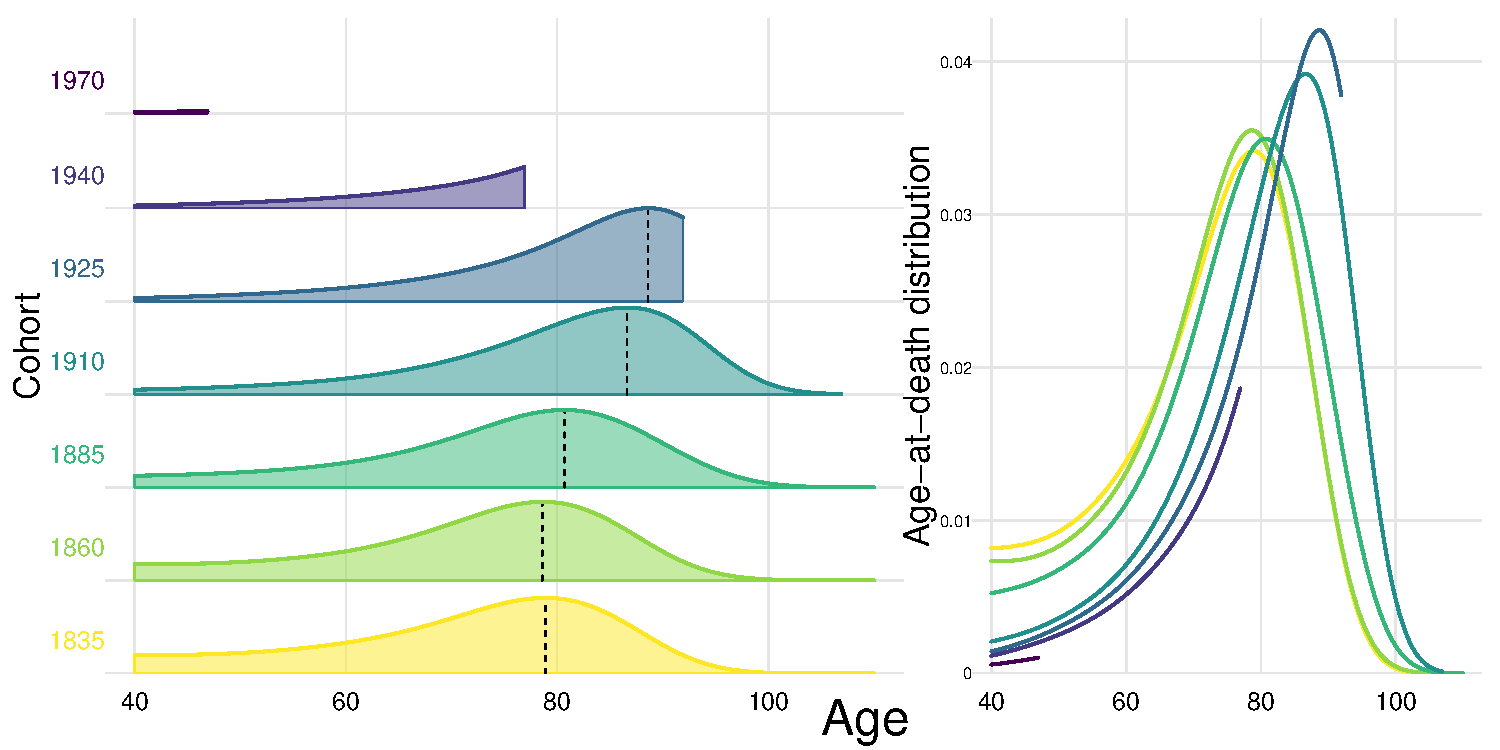
\includegraphics[scale=0.53]{./Ch3/F1.pdf}	
		\caption{Death rates in logarithmic scale (left panel) and corresponding age-at-death distributions (right panel) for Japanese females in 1960 (blue line) and 2010 (green line). Data have been smoothed for illustrative purposes. Source (Figs.~\ref{Fig:MxLxDxCurves}-\ref{Fig:DxFore}): Authors' calculations based on data from the \cite{HMD}.\label{Fig:MxLxDxCurves}}			
	\end{center}
\end{figure}

The graph clearly shows the modal age at death (the age at which most of the deaths occur) and its significant shift to the right from 1960. Moreover, the spread of the distribution provides an indication of the lifespan variability. A decrease in variability over time can be observed directly (the distribution in 2010 is taller and more compressed than the one in 1960) and can be measured, for example with the interquartile range of life-table ages at death or the Gini coefficient \citep[for comprehensive reviews, see][]{wilmoth1999rectangularization,van2013perturbation}. Age-at-death distributions thus provide key insights on longevity and lifespan variability that cannot be grasped directly from either mortality rates or the survival function.

Trends in longevity and lifespan variability across countries and time have been extensively investigated in the demographic literature. While almost universal agreement has been reached on the remarkable and sustained increase in longevity over the last two centuries in more economically developed countries, assessments of trends of lifespan variability depend, at least to some extent, on the measure being used \citep[see, for
example,][pp.~314-318]{shkolnikov2003gini}. A comprehensive review of the findings is beyond the scope of this paper; however, in broad terms, it has been shown that increases in longevity are associated with decreasing variability of deaths in long-lived industrialized human societies \citep{smits2009length,vaupel2011life} and across the full range of human experience, for both males and females \citep{colchero2016emergence}. 

Despite being well suited to portray mortality patterns and to study longevity and lifespan variability, age-at-death distributions have generally been neglected in modelling and forecasting. Only a few attempts have been made to explicitly use them to forecast mortality. Some efforts have been made using Compositional Data Analysis: \cite{oeppen2008coherent} and \cite{bergeron2017coherent} suggested a modified version of the Lee-Carter model \citep{lee1992modeling}, in which the life-table death distribution (instead of the logarithm of death rates) is forecast using Principal Component Analysis. Furthermore, \cite{pascariu2019maximum} introduced a vector-autoregressive time series model to forecast a number of statistical moments of the distribution of deaths.

In this paper, we propose a novel methodology for modelling and forecasting adult mortality that is based on age-at-death distributions. Our model captures mortality dynamics by transforming the age axis of a reference "standard" distribution that is fixed over time. The transformation function is characterized by three parameters that describe changes in longevity and in lifespan variability, and it takes the form of a segmented linear function. For this reason, we call our model the \emph{Segmented Transformation Age-at-death Distributions}, or STAD, model. The total variability is divided into two components, the variability before and after the modal age at death; the model thus sheds light on the independent contribution of these two age ranges to the overall lifespan variability. The shifting and compression dynamics of mortality are captured and disentangled by the three parameters of the model, and mortality forecasts are derived from extrapolation of the parameters using time series models. 

This paper is organized as follows. In Section \ref{Sec:Ch3sec2}, we review the methodology that we propose in this article. We start by introducing the STAD model in Section \ref{Subsec:Ch3subsec2.1}; then, we show how to choose and compute an appropriate standard distribution in Section \ref{Subsec:Ch3subsec2.2}. Section \ref{Subsec:Ch3subsec2.3} presents the data and the smoothing procedure that we employ in our analyses, while the methods for estimating and forecasting the STAD parameters are presented in Section \ref{Subsec:Ch3subsec2.4}. In Section \ref{Sec:Ch3sec3}, we provide an illustration of our methodology by estimating and forecasting female mortality in four high-longevity countries, namely Sweden, Japan, France and Denmark. In Section \ref{Subsec:Ch3subsec3.1}, we evaluate the goodness-of-fit of the STAD model by comparing the estimated mortality pattern with the observed data, both graphically and formally. In Section \ref{Subsec:Ch3subsec3.2}, we assess the accuracy of the STAD forecasts by performing three out-of-sample validation exercises with forecast horizons of 10, 20 and 30 years, respectively. Finally, in Section \ref{Subsec:Ch3subsec3.3}, we show the mortality forecasts of the four countries up to 2040. In each section, we use data retrieved from the \cite{HMD}, and we compare our forecasts with those of the Lee-Carter model and its most well-known variants \citep{shang2011point}. In Section \ref{Sec:Ch3sec4}, we discuss the results and conclude. 


\section{Methods}\label{Sec:Ch3sec2}

\subsection{The Segmented Transformation Age-at-death Distributions Model}\label{Subsec:Ch3subsec2.1}

For ease of presentation, we consider here only two adult age-at-death distributions, defined on the age range 30-110: a "standard" distribution $f(x)$, and an observed distribution $g(x)$, where $x$ denotes age. The functional form of the distributions does not have any restrictions, as it can be parametric, nonparametric or an actual age-at-death distribution. Let $t(x;\bm{\theta})$ be a transformation function of the age axis and a set of parameters $\bm{\theta}$ such that the observed distribution conforms to the standard on the  warped axis, that is:
% 
\begin{equation}\label{eq_gxftx}
g(x) = f\left[t(x;\bm{\theta})\right] \, \, 
\end{equation}
%
i.e.~the distribution $g(x)$ is derived from altering the age axis of the standard distribution $f(x)$. Our aim is to find a transformation function that describes mortality developments in a parsimonious and rigorous manner. Given this purpose, we propose a transformation function $t(x;\bm{\theta})$ that depends only on (i) the changes in modal ages at death between $f(x)$ and $g(x)$; (ii) the differences in the variability of deaths of $f(x)$ and $g(x)$ before and (iii) after their modal ages. 

Formally, let $s = M^{g} - M^{f}$ be the difference between the modal ages at death of $g(x)$ and $f(x)$. Then, the transformation function of the proposed \emph{Segmented Transformation Age-at-death Distributions} (STAD) model can be expressed as follows:  
\begin{equation}\label{eqtx}
t(x;s,b_{L},b_{U}) = \left\{ \begin{array}{ll}
M^{f} + b_{L} \, (x - s - M^{f}) \quad & \mathrm{if} \; x \leq M^{g} \\
M^{f} + b_{U} \, (x - s - M^{f}) \quad & \mathrm{if} \; x >  M^{g} \\
\end{array}
\right.
\end{equation}
where the non-negative coefficients $b_{L}$ and $b_{U}$ denote the change in the variability from $f(x)$ to $g(x)$ before and after their modes, respectively.    

In words, the transformation function $t(x;s,b_{L},b_{U})$ takes the form of a segmented linear model that breaks at the value of $M^{g}$. The slopes of each linear part $b_{L}$ and $b_{U}$ capture the amount of expansion/reduction of variability of deaths needed before and after $M^{g}$, respectively, so that $f(x)$ fit the observed distribution $g(x)$. Changes in the mortality pattern of $g(x)$ with respect to $f(x)$ can thus be concisely described by the three parameters $s$, $b_{L}$ and $b_{U}$. The three parameters have a very important demographic interpretation, as they directly capture the shifting and compression dynamics of mortality changes observed during the twentieth century \citep{fries1980aging,wilmoth1999rectangularization,bongaarts2005long,canudas2008modal}.  

A schematic overview of the STAD model is useful to better explain the segmented linear transformation and the shifting/compression mortality dynamics. Figure \ref{Fig:TransfExample} presents the effects of applying the segmented function $t(\cdot)$ to a given standard distribution $f(x)$ (black line of the graphs). When a simple shift is adopted (red line of the graphs), the standard distribution is only moved to the right (as in the graph, or to the left), maintaining the same variability (as measured by the variance, if the age range is shifted too) before and after the modal age at death. This is a special case of Eq.~\eqref{eqtx} in which both $b_{L}$ and $b_{U}$ are equal to 1 and the transformation function becomes: $t(x;s) = x - s$. As such, the parameter $s$ regulates the \textit{shifting} dynamic of mortality.

\begin{figure}[!ht]
	\begin{center}
		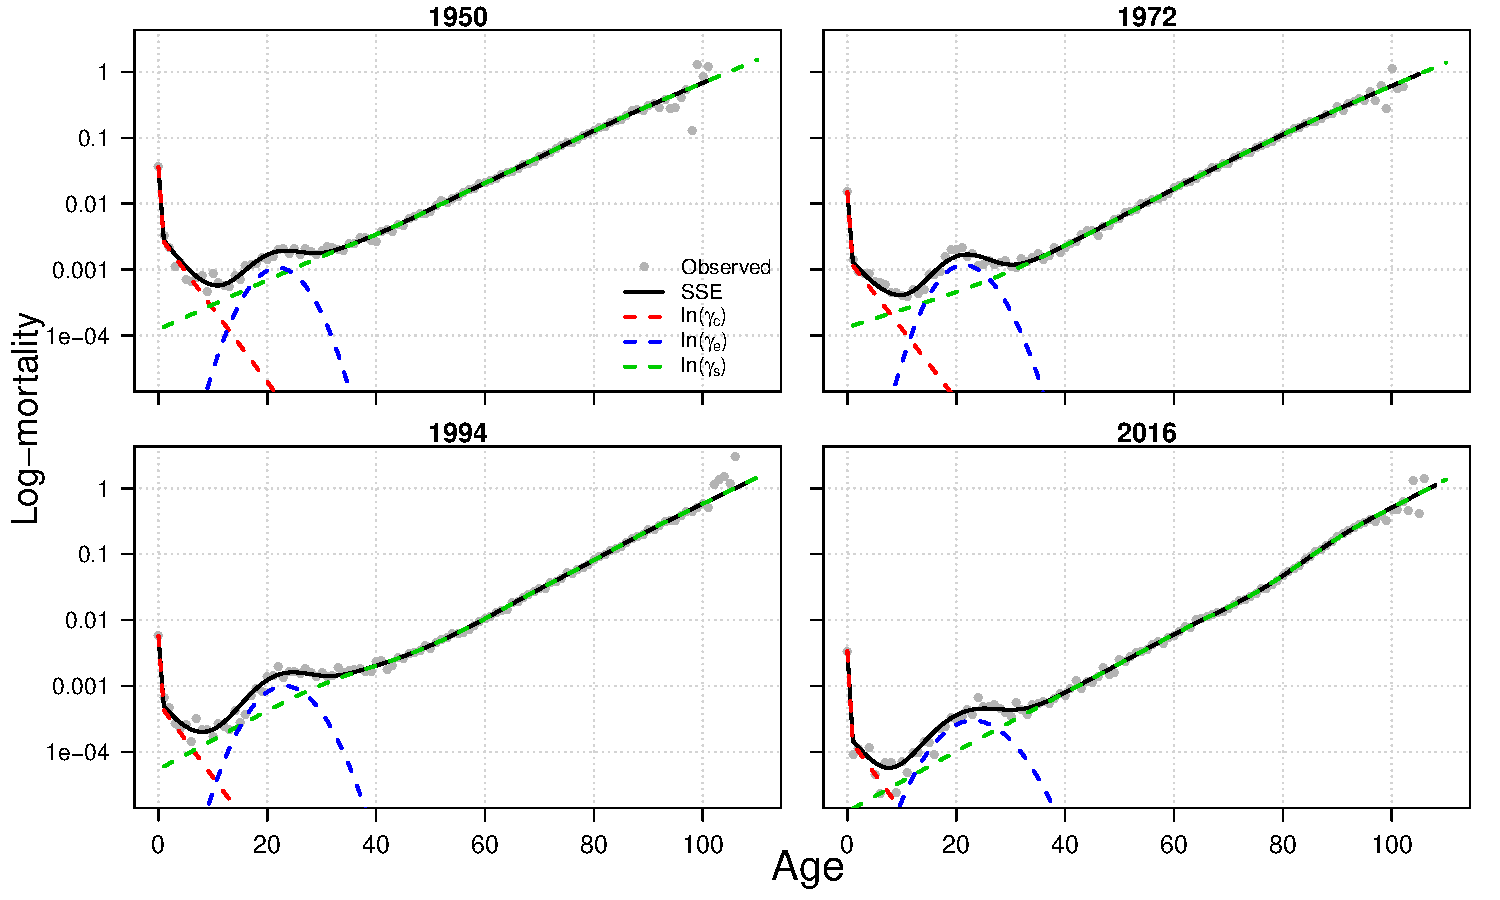
\includegraphics[scale=0.53]{./Ch3/F2.pdf} 
		\caption{A schematic overview of the effects of transforming the
			age axis using the \emph{Segmented Transformation Age-at-death
			Distributions} model.\label{Fig:TransfExample}}    
	\end{center}
\end{figure}

More flexible scenarios can be achieved by modifying the values of $b_{L}$ and $b_{U}$ that act jointly with the shifting parameter $s$. When $b_{L}$ and $b_{U}$ are greater than 1, the ages before and after the mode of $g(x)$ are shrunk, and variability in ages at death is decreasing with respect to $f(x)$. On the other hand, when $b_{L}$ and $b_{U}$ are smaller than 1, the ages before and after $M^{g}$ are expanded, so that age at death variability increases compared to the standard. These two parameters thus capture the \textit{compression} dynamic of mortality in two age ranges, as they expand or reduce the variability of deaths before and after the mode. In the example presented in Figure \ref{Fig:TransfExample}, the ages before the mode are shrunk ($b_{L} > 1$) and the ages above are expanded ($b_{U} < 1$), so that the resulting variability is reduced before the mode and increased above the mode with respect to the standard (purple line of the graphs).  

Interestingly, the STAD model is able to capture two limit scenarios of mortality patterns. On one hand, the complete rectangularization of the survival curve can be obtained by letting $b_{L}$ and $b_{U}$ go to infinity. In this case of maximum compression, the death distribution becomes a probability mass function with probability one at the modal age at death, and lifespan variability is zero as all individuals die at the same age. On the other hand, the case of maximum expansion is achieved when $b_{L}$ and $b_{U}$ are equal to zero. In this case, the death distribution becomes a uniform distribution, and lifespan variability is maximized.

Finally, it should be noted that despite introducing a break point at $M^{g}$ in $t(\cdot)$, there is no disruption at the mode of the transformed distribution. This can be seen in the left panel of Figure \ref{Fig:TransfExample}: although $b_L$ and $b_U$ have different values, the segmented linear transformation is continuous at the age $M^{g}$, which remains the modal age of the warped distribution depicted in purple.    

\subsection{The standard distribution}
\label{Subsec:Ch3subsec2.2}

The standard distribution of the STAD model has a very important role: every observed distribution in the time period analysed can be derived from applying the transformation function $t(\cdot)$ with appropriate parameters $s$, $b_L$ and $b_U$ to the standard. As such, the standard is a "reference", or background, distribution that should contain the representative features of the observed distributions. The STAD model can thus be thought as a relational model \citep{brass1971scale}, and therefore choosing a suitable standard is both desirable and necessary for improving the fit of the model.  

A first approach to select the standard could be to take a summary
measure (such as the mean or the median) of a series of observed
distributions. However, this would lead to a bias, as depicted in the
left panel of Figure \ref{Fig:Standard}. Let us consider, for
simplicity, only two observed distributions $g_{1}(x)$ and $g_{2}(x)$. Taking
the simple mean of them results in a standard $f(x)$ with a fairly
unrealistic shape that does represent neither mortality age-pattern in
$g_{1}(x)$ nor in $g_{2}(x)$. The reason for this behavior is that $f(x)$
conflates age segments that are positioned before and after 
the mode in the two observed distributions: the decreasing part of
$g_1(x)$ after its mode is averaged with the increasing part of $g_2(x)$
before its mode. 

\begin{figure}[!ht]
	\begin{center}
		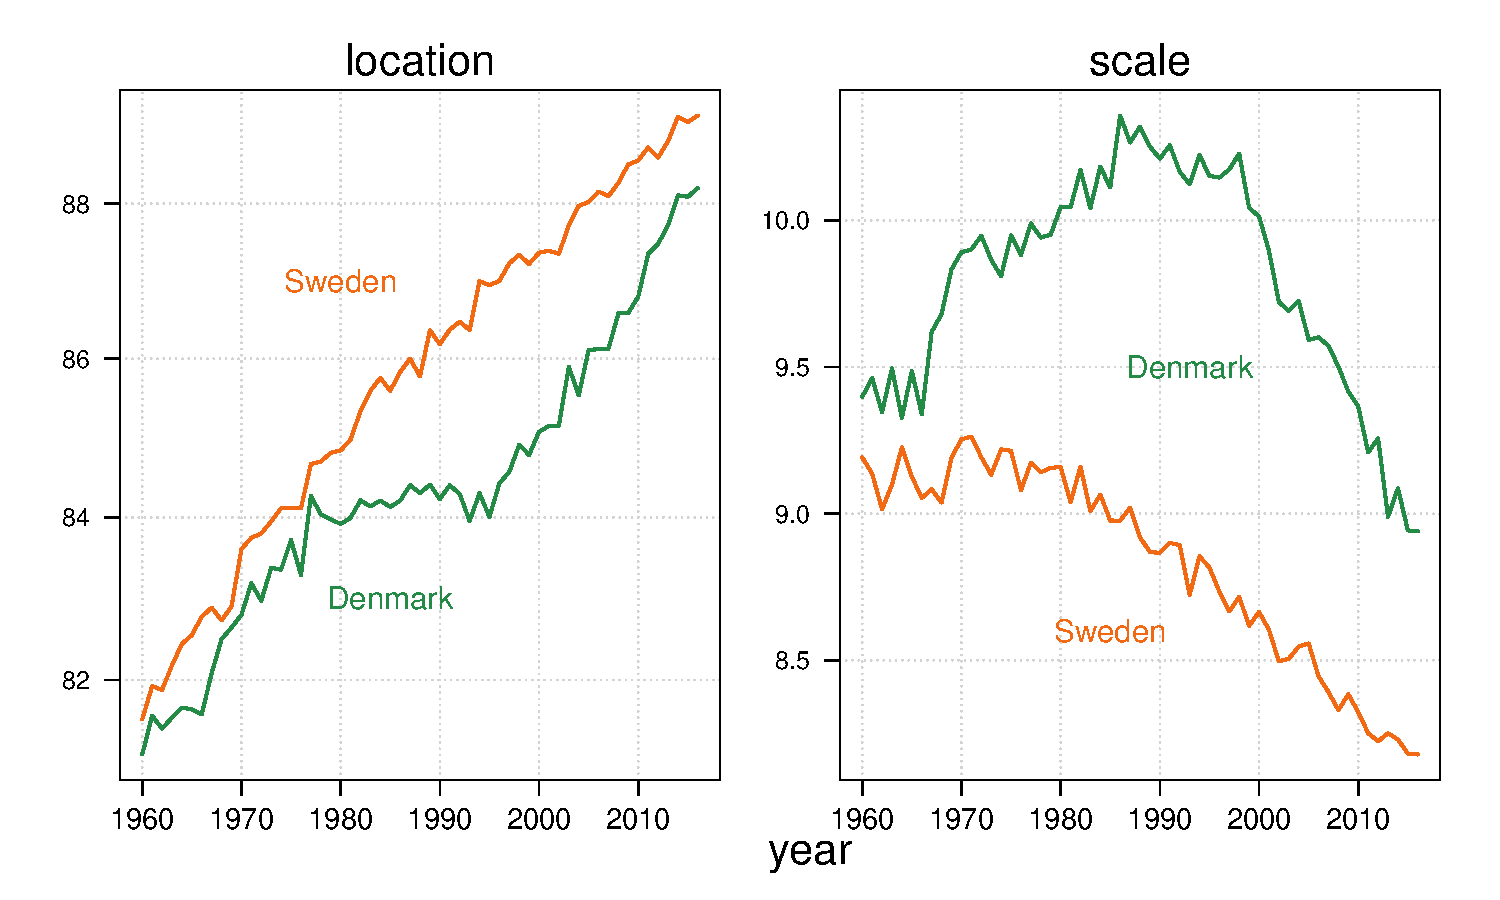
\includegraphics[scale=0.51]{./Ch3/F3.pdf}   
		\caption{Standard distributions $f(x)$ (black line) computed as
			mean of the observed densities $g_{1}(x)$ and $g_{2}(x)$ (left panel) and
			as mean of the  observed $g_{1}(x)$ and aligned $\breve{g}_{2}(x)$ (right
			panel).\label{Fig:Standard}}    
	\end{center}
\end{figure}

In order to avoid this problem, we first transform the observed densities to line up their qualitative features. Specifically, we shift the densities so that their modal ages at death are equal to the mode of the first observed density, maintaining their variability unchanged. This procedure is known as \emph{landmark registration}, and is commonly used in Functional Data Analysis \citep{ramsay2005FDA} with the aim of "eliminating uninteresting differences in functions so that the remaining functional variation is (more) completely concerned with the differences of interest" \citep[p.~88]{clarkson2005fdamanual}. Here, by aligning the distributions we remove the differences in the mode (that are already captured by the parameter $s$), and we focus on the differences in their variability. 

Having aligned the observed distributions, the standard distribution is then computed as the mean of the aligned distributions. In the right panel of Figure \ref{Fig:Standard}, $g_{2}(x)$ is shifted to the left such that its mode aligns with that of $g_{1}(x)$, and $f(x)$ is computed as the mean of the observed $g_{1}(x)$ and the aligned $\breve{g}_{2}(x)$. This registered mean provides a better representation of the two densities: the shape of $f(x)$ is more realistic, its mode is equal to those of $g_1(x)$ and $\breve{g}_{2}(x)$, and its variability is the average variability of the two distributions.  

Finally, for capturing any type of shifting, we need to extend the age-support of the standard distribution, $f(x)$. For example, in the simple shift case in Figure \ref{Fig:TransfExample}, the value of the shifted distribution (red line) at age 30 is equal to the value of the expanded standard (black line) evaluated at $x-s$, i.e.~beyond the original 30-110 age range. We can carry out this extension since we assume that the senescent (older adult) component of mortality is independent from the juvenile and younger adult ones. We achieve this task by means of nonparametric techniques: we extrapolate the mortality age-pattern of $f(x)$ without any rigid assumption on its form. 

\subsection{Data and estimation of the standard distribution}\label{Subsec:Ch3subsec2.3}

We apply the STAD model to the female population of four high-longevity countries, namely Sweden, Japan, France and Denmark. Whereas Sweden was selected as benchmark population for its high standard in data quality even at most advanced ages \citep{vaupel1994longer,wilmoth1996extreme}, Japan and France have repeatedly been identified as countries where average lifespan is very high \citep{wilmoth1996extreme,oeppen2002broken,cheung2007increase,canudas2008modal,canudas2010three,horiuchi2013modal}. Finally, Denmark showed a rather peculiar mortality trajectory: among the highest longevity countries until the 1980s, this population was characterized by a stagnation of life expectancy in the last two decades of the twentieth century \citep{christensen2010divergent, lindahl2016did, lindahl2016rise}. In order to test the fitting and forecasting performance of our STAD model, we apply it on these diverse mortality developments.

As already mentioned, our interest is restricted to the senescent (older adult) component of mortality. We thus start our analyses from age 30. Furthermore, we aim to forecast mortality up to 2040, hence we choose 1980-2014 as the fitting period. This allow us to study the most recent mortality developments \citep[excluding improvements in the 1970s due to the cardiovascular revolution,][]{vallin2004convergences} while keeping the length of the fitting period long enough to forecast twenty-six years ahead. 

Specifically, data are obtained from the \citeauthor{HMD} (HMD, \citeyear{HMD}) and they are observed death counts $D_{x,y}$ and  exposure-to-risk $E_{x,y}$, classified by age at death, $x=30,\ldots, 110+$, and year of death, $y=1980, \ldots, 2014$. Moreover, in the following,  we assume that the number of deaths at given age $x$ and year $y$ follows a Poisson distribution
\citep{brillinger1986biometrics}: 
%
\begin{equation}\label{Eq:Ch3Poisson}
D_{x,y} \sim \mathcal{P}(E_{x,y} \; \mu_{x,y}) 
\end{equation}
%
where $\mu_{x,y}$ is the hazard function, whose estimation is the object of any mortality model.

As presented in Section~\ref{Subsec:Ch3subsec2.1}, the STAD model is expressed in continuous notation. In order to use the model with observed discrete mortality data, a nonparametric smoothing approach is useful, so that mortality can be evaluated at any finer scale of the age axis, practically at a continuous level. In addition, the smoothing procedure avoids imposing rigid parametric mortality structures that could contribute to misleading outcomes. 

The first step in the STAD model consists in extracting the standard distribution as mean of the aligned observed distributions with respect to the first modal age at death (1980 in our case). To perform this task, we need to compute age-at-death distributions and associated modes for each year. Instead of modelling directly the life-table deaths, we make use of the assumption in Eq.~\eqref{Eq:Ch3Poisson} and smooth actual death counts using a $P$-splines approach and exposures as offset \citep{eilers1996flexible,camarda2012mortalitysmooth}. The advantage of this approach is twofold. First, we use an objective selection of the amount of smoothing based on the Bayesian Information Criterion \citep[BIC,][see Appendix \ref{Subsec:Ch3appA}]{schwarz1978estimating}. This approach accounts for the size of the population analysed due to the Poisson assumption of death counts \citep{brillinger1986biometrics}. In contrast, smoothing life-table deaths is more subjective, because the optimal degree of smoothing depends on the life-table radix: given the same age-specific mortality pattern, higher starting radices are associated with a lower amount of smoothing. Second, we smooth observed rather than life-table deaths because the latter are constructed from adjusted death rates, as the HMD employs a logistic function for ages 80 and above \citep{Wilmoth2007}. 

Having smoothed mortality, we can derive the corresponding smooth
age-at-death distributions: $g(x)=\mu(x)\,l(x)$, where the survival
function $l(x)$ can be computed numerically from the smooth death
rates, evaluated at extremely fine grid. As shown in
\citet{ouellette2011changes}, this procedure further allows us to directly extract modal ages at death for each year, $M^{y}$. 
Given the series of $M^{y}$, we already have the
estimate of the shifting parameter for each year, i.e.~the difference in modal
ages at death between a given year and the first year,  $s_{y} = M^{y}-M^{1980}$.

Using estimates from the $P$-splines approach, we can express the smooth observed distribution for year $y$ as follows:
% 
\begin{equation}\label{Eq:Ch3gx_smooth}
g_{y}(x) = \exp\left[ \bm{B}(x) \, \bm{\beta}_{y} \right]
\end{equation}
%
where $\bm{B}(x)$ is a basis of equally spaced $B$-splines over ages $x$ and $\bm{\beta}_{y}$ are coefficients specific to the distribution $g_{y}(x)$. The estimated series of $s_{y}$ allow us to align all distributions by simply re-evaluating the $B$-splines basis in Eq.~\eqref{Eq:Ch3gx_smooth} on the shifted age axes:
%
\begin{equation}
\breve{g}_{y}(x) = \exp\left[ \bm{B}(x - s_{y}) \, \bm{\beta}_{y}
\right] \, . 
\end{equation}
%
The standard distribution $f(x)$ can then be obtained by averaging the
aligned observed distributions. Again, the standard distribution can
be expressed as a linear combination of $B$-splines over $x$ and new
coefficients $\bm{\beta}_{f}$ specific to
$f(x)$:
% 
\begin{equation}
f(x) = \exp\left[ \bm{B}(x) \, \bm{\beta}_{f} \right] \, .
\end{equation}
%
It is noteworthy that the coefficients $\bm{\beta}_{f}$ contain all the representative age-specific mortality features that we will use for describing mortality developments
over time, except shifting and compression/expansion that are captured
by the parameters $s$, $b_{L}$ and $b_{U}$.

\subsection{Estimation and forecast of the STAD parameters}\label{Subsec:Ch3subsec2.4}

Given the estimated standard distribution $f(x)$, the model parameters can
then be estimated. For each year $y$, we seek to find a set of three parameters
$\left[s_{y}, b_{L,y}, b_{U,y} \right]$ that produces a transformation of the
age axis defined in Eq.~\eqref{eqtx} such that the mortality pattern of the transformed
standard $f\big(t(x; s_{y}, b_{L,y}, b_{U,y})\big)$ fits the observed data.   

Whereas the shifting parameters $\hat{\bm{s}}$ are readily estimated within
the alignment procedure, estimation of the
compression/expansion parameters is achieved by maximum likelihood. Based on the Poisson assumption in Eq.~\eqref{Eq:Ch3Poisson}, the parameters $\hat{\bm{b}}_{L}$ and $\hat{\bm{b}}_{U}$ are obtained by maximizing
the following log-likelihood:   
\begin{equation}\label{Eq:Ch3loglike}
\ln \, \mathcal{L}\left(b_{L,y},b_{U,y} | \, D_{x,y} , E_{x,y} , \hat{s}_{y} , \bm{\beta}_{f}
\right) \propto \sum_{x} \left \{  D_{x,y} \,
\ln \left ( \mu^{\texttt{STAD}}_{x,y}  \right ) - E_{x,y}
\, \mu^{\texttt{STAD}}_{x,y} \right \}  
\end{equation}
for $y=1980,\ldots,2014$, where $\mu^{\texttt{STAD}}_{x,y}$ denotes
the hazard function corresponding to the estimated segmented
distribution of the STAD model.

On one hand, data and log-likelihood are expressed in
terms of deaths, exposures and hazard. On the other hand, the STAD model is
described in terms of distributions. This is not an issue because, as we already introduced in Section \ref{Sec:Ch3sec1}, hazard and distributions are complementary: knowing one of them allows to directly and uniquely derive the other. As such, the estimated $\hat{\bm{b}}_{L}$ and $\hat{\bm{b}}_{U}$ are the parameters that produce a transformed segmented distribution $f\left[\hat{t}(\cdot)\right]$ whose corresponding hazard $\mu^{\texttt{STAD}}$ maximizes Eq.~\eqref{Eq:Ch3loglike}.  

A general-purpose numerical optimizer works well for maximizing Eq.~\eqref{Eq:Ch3loglike} and estimate $\hat{\bm{b}}_{L}$ and $\hat{\bm{b}}_{U}$. Routines for estimating the standard distribution as well as the
transformation function for the age axis based on maximum likelihood
were implemented in \texttt{R} \citep{Rcite} and are available in the supplementary material.

Having estimated the parameters over years, it is
possible to model their time series: mortality forecasts are then
obtained by extrapolation of the STAD parameters and the time-fixed
standard distribution. In other words, we assume that mortality developments can
be well approximated by a standard age-pattern and time-indexes
capturing mortality dynamics in shifting and compression/expansion. 

Among the numerous approaches available for time series modelling and
forecasting, we combine univariate and multivariate models to describe and forecast the time evolution of the three parameters. Since the shifting and compression/expansion dynamics act independently in the STAD model, i.e.~changes in $s$ do not affect $b_{L}$ and $b_{U}$ and vice versa (as shown in Figure \ref{Fig:TransfExample}), we treat $s$ separately from the two $b$ parameters. For $s$, we choose the standard class of univariate autoregressive integrated moving average models, ARIMA($p$, $d$, $q$). The three parameters of the ARIMA are chosen among different combinations, using an automatic step-wise algorithm based on the minimization of the corrected Akaike Information Criterion
\cite[the package default, see][]{hyndman2008automatic}.

Changes between the two $b$ parameters could instead be correlated: for example, if a mortality change would maintain the same overall lifespan variability but compress the ages before the mode, then $b_{U}$ would necessarily need to expand (or vice versa). As such, we favour a multivariate approach to model $b_{L}$ and $b_{U}$, as this takes into account the interrelationship \textit{within} and \textit{between} the two series. Consequently, for the $b$ parameters we employ a vector autoregressive (VAR) model, which is the multivariate generalization of univariate autoregressive time series models \citep{hamilton1994time}. We perform model selection, estimation and diagnostic tests using the \texttt{R} package \texttt{vars} \citep{pfaff2008analysis,pfaff2008var}. Forecasts of all three parameters are then computed with the \texttt{forecast} package \citep{hyndman2018forecastR}.


\section{Results}\label{Sec:Ch3sec3}

\subsection{Observed versus fitted data}\label{Subsec:Ch3subsec3.1}

We fit the STAD model to the female population of Sweden, Japan, France and Denmark using data described in Section \ref{Subsec:Ch3subsec2.3}. The estimated standard distribution and parameters $\hat{\bm{s}}$, $\hat{\bm{b}}_{L}$ and $\hat{\bm{b}}_{U}$ allow us to derive the mortality pattern over time in each country. To assess the goodness-of-fit of the STAD, we investigate two summary measures of the mortality pattern that answer the questions outlined in Section \ref{Sec:Ch3sec1}: remaining life expectancy at age 30 ($e_{30}$, Q1) and the Gini coefficient at age 30 ($G_{30}$, Q2). The former measure is computed using standard demographic methods \citep{preston2001demogr}, while the latter is derived from the formula in \cite{shkolnikov2003gini}.

Figure \ref{Fig:LifeExpFit} shows the observed and fitted $e_{30}$ and $G_{30}$ for females in the four countries over the years 1980-2014. The graphs show that the STAD model performs very well in terms of goodness-of-fit. In the top graphs, the actual and fitted $e_{30}$ are always very close to each other, with a small loss of goodness-of-fit in some years for Danish females, probably due to their peculiar trend \citep{christensen2010divergent,lindahl2016did,lindahl2016rise}. Similarly, the goodness-of-fit for $G_{30}$ is satisfactory, with small discrepancies in the first years for Denmark and in the last years for Japan and France.	

\begin{figure}[!ht]
	\begin{center}
		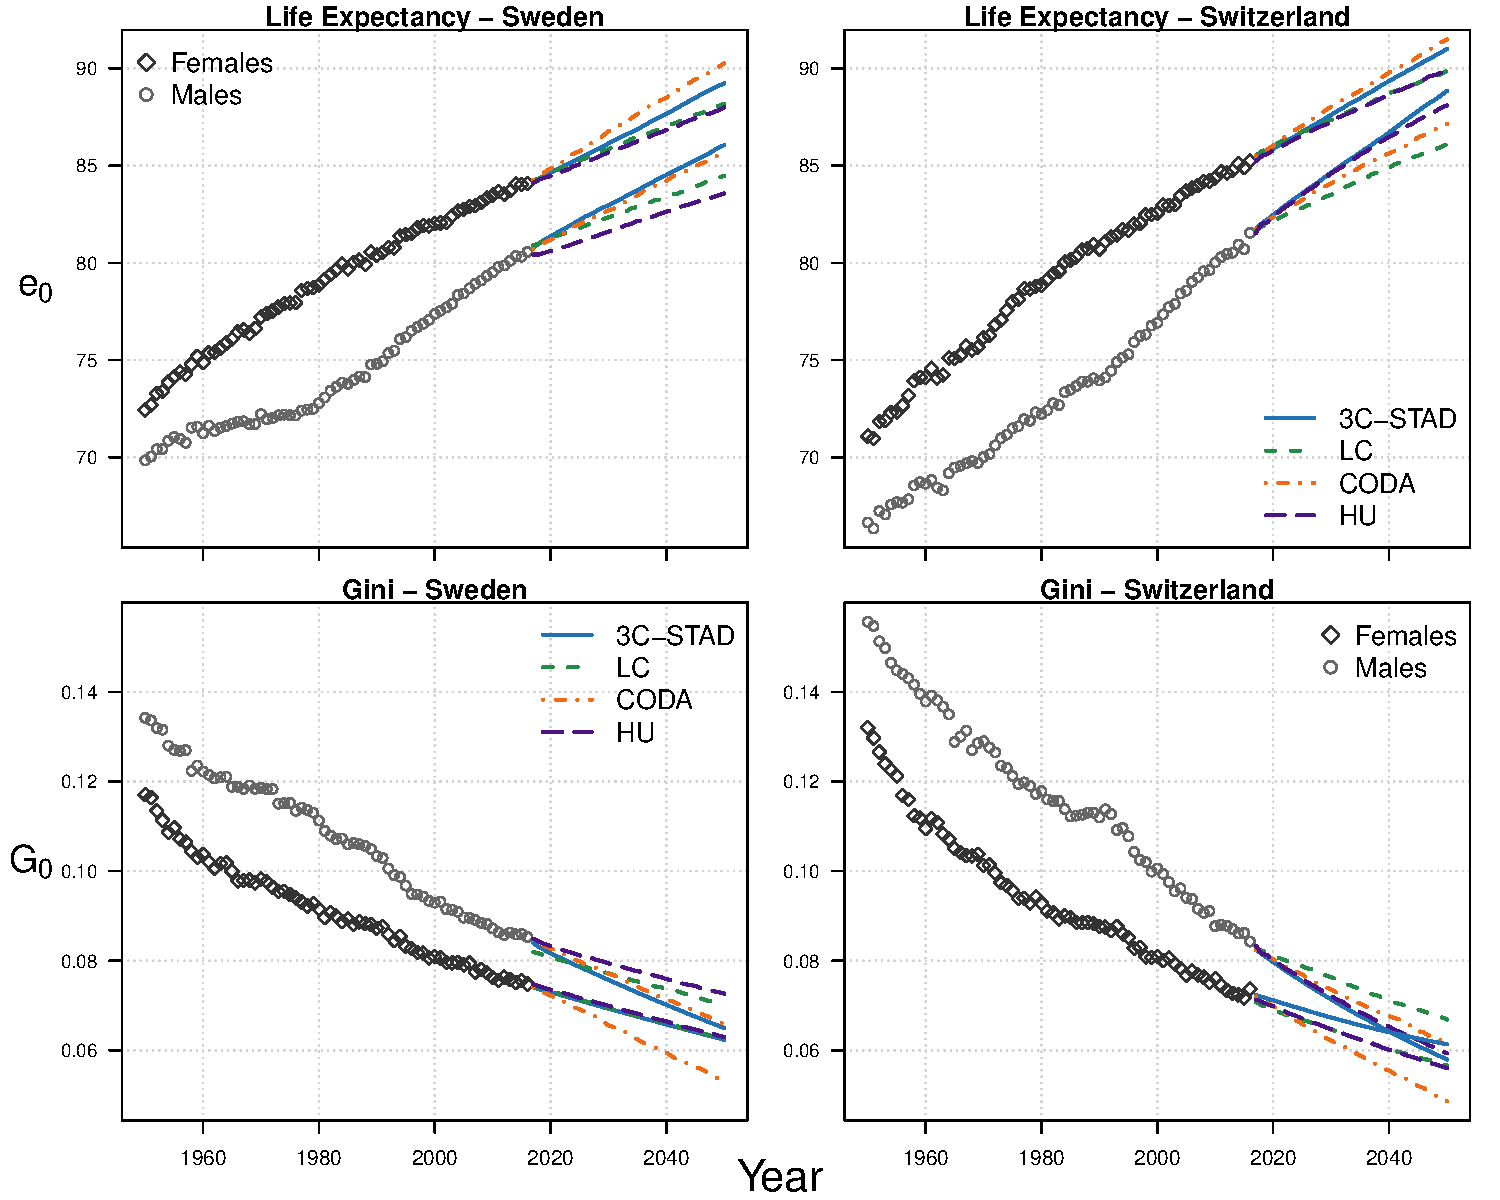
\includegraphics[scale=0.77]{./Ch3/F4.pdf}
		\caption{Comparison of observed (points) and STAD fitted (crosses)
			remaining life expectancy at age 30 ($e_{30}$, top graphs) and Gini coefficient at age 30 ($G_{30}$, bottom graphs) for females in Sweden,
			Japan, Denmark and France during
			1980-2014.\label{Fig:LifeExpFit}}		
	\end{center}  
\end{figure}

In order to perform a more formal statistical assessment of the goodness-of-fit of the STAD model beyond this graphical investigation, we compare the fit of the STAD with the standard \citeauthor{lee1992modeling} (LC, \citeyear{lee1992modeling}) model and its variants, estimated on the same ages and years. We employ the Bayesian Information Criterion \citep[BIC,][]{schwarz1978estimating} to measure model differences in terms of trade-off between model parsimony and accuracy (see Appendix \ref{Subsec:Ch3appA} for additional details and computational procedure).

In the following, we consider all the variants of the LC model that can be readily estimated with available packages in \texttt{R}. In particular, these models are: \citeauthor{lee2001evaluating} (LM, \citeyear{lee2001evaluating}), \citeauthor{booth2002applying} (BMS, \citeyear{booth2002applying}), \citeauthor{brouhns2002poisson} (BDV, \citeyear{brouhns2002poisson}), \citeauthor{hyndman2007robust} (HU, \citeyear{hyndman2007robust}),
robust \citeauthor{hyndman2007robust} (HUrob, \citeyear{hyndman2007robust}) and weighted \citeauthor{hyndman2007robust} (HUw, \citeyear{hyndman2007robust}) \citep[for a concise review of these models, see][]{shang2011point}. The LC variants have been fitted using the \texttt{R} packages \texttt{demography} and \texttt{StMoMo}  \citep{demogRpackage,StMoMoRpackage}. For the HU, HUrob and HUw model, we chose the \texttt{demography} package default value of six principal components, as suggested by \cite{hyndman2008stochastic} and employed by \cite{shang2011point}.

Table \ref{Table:BIC} shows the BIC values of the STAD and LC variants in the four countries (values of the Deviance and Effective Dimension are reported in Appendix \ref{Subsec:Ch3appB}). The STAD is chosen over the other models in Sweden and Denmark.  For Japan, the standard \citeauthor{hyndman2007robust} method is the best fitting model, and the Poisson variant of the LC model (BVD) is preferred for France. 

\begin{table}[!ht]
	\centering
	
	\begin{tabular}{lR{1.4cm}R{1.4cm}R{1.2cm}R{1.2cm}R{1.4cm}R{1.4cm}R{1.4cm}R{1.4cm}}
		\toprule
		& \multicolumn{8}{c}{Model} \\ \cmidrule(rr){2-9} 
		Country & STAD & LC & LM & BMS & BDV & HU & HUrob & HUw           \\ 
		\rowcolor{my-grey}
		\midrule
		\belowrulesepcolor{my-grey}
		Sweden                   & \textbf{4276}          & 4699          &     4703     & 4674       & 4611 & 8871  & 9040    &   9018    \\ 
		
		Japan                    & 11053          & 11475                &     11818     & 11387       & 10790 & \textbf{10057}  & 10694    &   10981        \\
		\rowcolor{my-grey}
		France                   & 9141        & 7822                &     7951     & 7773       & \textbf{7663} & 9402  & 10132    &   9858 \\
		Denmark                  & \textbf{5332}          & 5613                     &     5604     & 5587       & 5485 & 9020  & 9397    &   9890           \\ 
		\bottomrule
	\end{tabular}
	\caption{BIC values of the STAD and LC model and variants for females aged 30-110+ in four countries during 1980-2014. Lower values of the BIC (in bold) correspond to a better model.}\label{Table:BIC}
\end{table}


\subsection{Out-of-sample validation}\label{Subsec:Ch3subsec3.2}
Before projecting mortality into the future, we first assess the
accuracy of the STAD forecasts by out-of-sample validation. In particular, we compare the observed versus the point and interval forecasts of the remaining life expectancy at age 30 ($e_{30}$), the Gini coefficient at age 30 ($G_{30}$), and the logged age-specific death rates over all ages and years ($\ln(m_{x,t})$). Lifespan disparity measures such as the Gini index are in fact important indicators to evaluate mortality forecasts \citep{bohk2017lifespan}.	

The procedure of dividing the observed dataset into two parts, the first for fitting the model, and the second for checking predictions, is very common in forecasting \citep{chatfield2000time}. Here, we perform three out-of-sample validation exercises: we fit the STAD and the \citeauthor{lee1992modeling}  variants to three periods of equal length: 1970-2004, 1960-94 and 1950-84. Then, we forecast mortality until 2014 in all scenarios, corresponding to three forecast horizons of 10, 20 and 30 years, respectively. We then compare the point and interval forecasts of $e_{30}$, $G_{30}$ and $\ln(m_{x,t})$ at each forecast year with the observed data. 

For the point forecast analysis, we employ the mean absolute error (MAE) as measure of forecast accuracy, following standard time series practice \citep{chatfield2000time}. In addition, we only compare the forecast accuracy of the STAD model with the first four LC variants: we do not consider the functional data models (HU, HUrob and HUw) because their better performance is partially due to the much higher number of parameters employed (about four and five times more parameters than the LC variants and the STAD, respectively. See Effective Dimension in Appendix \ref{Subsec:Ch3appB}).

Table \ref{Table:MAE_ALLyears} shows the point forecast accuracy as measured by the MAE of $e_{30}$, $G_{30}$ and $\ln(m_{x,t})$ for the STAD and four LC variants in the three out-of-sample scenarios as well as for the four countries. The results of this analysis show that the STAD forecasts are overall more accurate than the LC ones. Out of 36 indicators, the STAD model is the most accurate almost half of the times (16 indicators). The LM is the second best performer (9 indicators), followed by the BMS (6 indicators), the BDV (4 indicators), and the original LC model (1 indicator). 

% TABLE TOTAL: 10, 20, 30 YEARS
\begin{table}[!ht]
	\centering
	\small
	\begin{tabular}{llcrR{1.3cm}R{1.3cm}R{1.3cm}R{1.3cm}}
		\toprule & & & \multicolumn{5}{c}{Model} \\ \cmidrule{4-8} 
		Country $\quad$ &  Test period &   Measure     &  STAD          & LC            & LM            & BMS           & BDV           \\ 
		\midrule
		%		\hhline{~~~|-----|} 
		
		% % SWEDEN
		
		\rowcolor{my-white} 
		\multicolumn{1}{l|}{\cellcolor{my-white}}    &     \multicolumn{1}{c|}{\cellcolor{my-white}}                 & \multicolumn{1}{c|}{\cellcolor{my-white}$e_{30}$} & 0.11          & 0.11          & 0.09          & 0.08          & \textbf{0.08} \\
		\rowcolor{my-white} 
		\multicolumn{1}{l|}{\cellcolor{my-white}}    &     \multicolumn{1}{c|}{\cellcolor{my-white}}                 & \multicolumn{1}{c|}{\cellcolor{my-white}$G_{30}$} & 0.17          & \textbf{0.06}          & 0.06          & 0.06          & 0.07 \\
		\rowcolor{my-white} 
		\multicolumn{1}{l|}{\cellcolor{my-white}} & \multicolumn{1}{c|}{\multirow{-3}{*}{\cellcolor{my-white}10y}} & \multicolumn{1}{c|}{\cellcolor{my-white}$\ln(m_{x,t})$}      & \textbf{0.10} & 0.12 & 0.12          & 0.12 & 0.11 \\ 
		\hhline{~|-------|}
		\rowcolor{my-grey} 
		\multicolumn{1}{l|}{\cellcolor{my-white}}    &         \multicolumn{1}{c|}{\cellcolor{my-grey}}             & \multicolumn{1}{c|}{\cellcolor{my-grey}$e_{30}$} & \textbf{0.25}           & 0.41           & 0.38           & 0.41          & 0.38 \\
		\rowcolor{my-grey} 
		\multicolumn{1}{l|}{\cellcolor{my-white}}    &      \multicolumn{1}{c|}{\cellcolor{my-grey}}                & \multicolumn{1}{c|}{\cellcolor{my-grey}$G_{30}$} & 0.41           & 0.15           & 0.21           & \textbf{0.15}           & 0.18 \\
		\rowcolor{my-grey} 
		\multicolumn{1}{l|}{\cellcolor{my-white}} & \multicolumn{1}{c|}{\multirow{-3}{*}{\cellcolor{my-grey}{20y}}} & \multicolumn{1}{c|}{\cellcolor{my-grey}$\ln(m_{x,t})$}      & \textbf{0.14}  & 0.16  & 0.18           & 0.16  & 0.16 \\ 
		\hhline{~|-------|}
		\rowcolor{my-white} 
		\multicolumn{1}{l|}{\cellcolor{my-white}}    &    \multicolumn{1}{c|}{\cellcolor{my-white}}                  & \multicolumn{1}{c|}{\cellcolor{my-white}$e_{30}$} & 0.87          & 0.81           & 0.80           & 0.80          &  \textbf{0.78} \\
		\rowcolor{my-white} 
		\multicolumn{1}{l|}{\cellcolor{my-white}}    &           \multicolumn{1}{c|}{\cellcolor{my-white}}           & \multicolumn{1}{c|}{\cellcolor{my-white}$G_{30}$} & 0.21      & 0.16       & \textbf{0.07}      & 0.16         & 0.12 \\
		\rowcolor{my-white} 
		\multicolumn{1}{l|}{\multirow{-9}{*}{\cellcolor{my-white}Sweden}} & \multicolumn{1}{c|}{\multirow{-3}{*}{\cellcolor{my-white}30y}} & \multicolumn{1}{c|}{\cellcolor{my-white}$\ln(m_{x,t})$}      & \textbf{0.15}  & 0.19  & 0.18     &  0.19  & 0.18 \\ \midrule
		
		
		% % % JAPAN
		
		\rowcolor{my-grey} 
		\multicolumn{1}{l|}{\cellcolor{my-grey}}    &     \multicolumn{1}{c|}{\cellcolor{my-grey}}                 & \multicolumn{1}{c|}{\cellcolor{my-grey}$e_{30}$} & 0.94          & 1.00         & 0.86 & \textbf{0.78} & 0.98 \\
		\rowcolor{my-grey} 
		\multicolumn{1}{l|}{\cellcolor{my-grey}}    &     \multicolumn{1}{c|}{\cellcolor{my-grey}}                 & \multicolumn{1}{c|}{\cellcolor{my-grey}$G_{30}$} & 0.11 & 0.55         & 0.14          & \textbf{0.07}          & 0.40 \\
		\rowcolor{my-grey} 
		\multicolumn{1}{l|}{\cellcolor{my-grey}} & \multicolumn{1}{c|}{\multirow{-3}{*}{\cellcolor{my-grey}10y}} & \multicolumn{1}{c|}{\cellcolor{my-grey}$\ln(m_{x,t})$}      & 0.12         & 0.21          & 0.12 & \textbf{0.11}          & 0.15 \\ \hhline{~|-------|}
		\rowcolor{my-white} 
		\multicolumn{1}{l|}{\cellcolor{my-grey}}    &         \multicolumn{1}{c|}{\cellcolor{my-white}}             & \multicolumn{1}{c|}{\cellcolor{my-white}$e_{30}$} & 0.86           & 0.35         & 0.35   & \textbf{0.31}  & 0.33 \\
		\rowcolor{my-white} 
		\multicolumn{1}{l|}{\cellcolor{my-grey}}    &      \multicolumn{1}{c|}{\cellcolor{my-white}}                & \multicolumn{1}{c|}{\cellcolor{my-white}$G_{30}$} & \textbf{0.74}  & 1.10          & 0.78           & 1.07          & 1.04 \\
		\rowcolor{my-white} 
		\multicolumn{1}{l|}{\cellcolor{my-grey}} & \multicolumn{1}{c|}{\multirow{-3}{*}{\cellcolor{my-white}{20y}}} & \multicolumn{1}{c|}{\cellcolor{my-white}$\ln(m_{x,t})$}      & \textbf{0.17}           & 0.25           & 0.20  & 0.25           & 0.22 \\ \hhline{~|-------|}
		\rowcolor{my-grey} 
		\multicolumn{1}{l|}{\cellcolor{my-grey}}    &    \multicolumn{1}{c|}{\cellcolor{my-grey}}                  & \multicolumn{1}{c|}{\cellcolor{my-grey}$e_{30}$} & 1.18           & 0.28          & \textbf{0.23}           & 0.45          & 0.32 \\
		\rowcolor{my-grey} 
		\multicolumn{1}{l|}{\cellcolor{my-grey}}    &           \multicolumn{1}{c|}{\cellcolor{my-grey}}           & \multicolumn{1}{c|}{\cellcolor{my-grey}$G_{30}$} & \textbf{1.06}         & 1.68           & 1.25           & 1.56           & 1.40 \\
		\rowcolor{my-grey} 
		\multicolumn{1}{l|}{\multirow{-9}{*}{\cellcolor{my-grey}Japan}} & \multicolumn{1}{c|}{\multirow{-3}{*}{\cellcolor{my-grey}30y}} & \multicolumn{1}{c|}{\cellcolor{my-grey}$\ln(m_{x,t})$}      & \textbf{0.22}  & 0.46  & 0.31    & 0.44  & 0.40 \\ \midrule
		
		% % FRANCE
		
		\rowcolor{my-white} 
		\multicolumn{1}{l|}{\cellcolor{my-white}}    &     \multicolumn{1}{c|}{\cellcolor{my-white}}                 & \multicolumn{1}{c|}{\cellcolor{my-white}$e_{30}$} & \textbf{0.13} & 0.44         & 0.30          & 0.35          & 0.36 \\
		\rowcolor{my-white} 
		\multicolumn{1}{l|}{\cellcolor{my-white}}    &     \multicolumn{1}{c|}{\cellcolor{my-white}}                 & \multicolumn{1}{c|}{\cellcolor{my-white}$G_{30}$} & \textbf{0.08} & 0.42          & 0.10          & 0.19          & 0.35 \\
		\rowcolor{my-white} 
		\multicolumn{1}{l|}{\cellcolor{my-white}} & \multicolumn{1}{c|}{\multirow{-3}{*}{\cellcolor{my-white}10y}} & \multicolumn{1}{c|}{\cellcolor{my-white}$\ln(m_{x,t})$}      & \textbf{0.07} & 0.12          & 0.07 & 0.10        & 0.11 \\ \hhline{~|-------|}
		\rowcolor{my-grey} 
		\multicolumn{1}{l|}{\cellcolor{my-white}}    &         \multicolumn{1}{c|}{\cellcolor{my-grey}}             & \multicolumn{1}{c|}{\cellcolor{my-grey}$e_{30}$} & 0.70  & 0.55           & \textbf{0.33}          & 0.47          & 0.47 \\
		\rowcolor{my-grey} 
		\multicolumn{1}{l|}{\cellcolor{my-white}}    &      \multicolumn{1}{c|}{\cellcolor{my-grey}}                & \multicolumn{1}{c|}{\cellcolor{my-grey}$G_{30}$} & 0.37  & 0.58           & \textbf{0.17}           & 0.54         & 0.51 \\
		\rowcolor{my-grey} 
		\multicolumn{1}{l|}{\cellcolor{my-white}} & \multicolumn{1}{c|}{\multirow{-3}{*}{\cellcolor{my-grey}{20y}}} & \multicolumn{1}{c|}{\cellcolor{my-grey}$\ln(m_{x,t})$}      & 0.13  & 0.16           & 0.13  & 0.16           & \textbf{0.12} \\ 
		\hhline{~|-------|}
		\rowcolor{my-white} 
		\multicolumn{1}{l|}{\cellcolor{my-white}}    &    \multicolumn{1}{c|}{\cellcolor{my-white}}                  & \multicolumn{1}{c|}{\cellcolor{my-white}$e_{30}$} & \textbf{0.21}  & 0.38           & 0.36          & 0.38       &  0.38  \\
		\rowcolor{my-white} 
		\multicolumn{1}{l|}{\cellcolor{my-white}}    &           \multicolumn{1}{c|}{\cellcolor{my-white}}           & \multicolumn{1}{c|}{\cellcolor{my-white}$G_{30}$} & \textbf{0.34}   & 0.45          & 0.36      & 0.45      & 0.45   \\
		\rowcolor{my-white} 
		\multicolumn{1}{l|}{\multirow{-9}{*}{\cellcolor{my-white}France}} & \multicolumn{1}{c|}{\multirow{-3}{*}{\cellcolor{my-white}30y}} & \multicolumn{1}{c|}{\cellcolor{my-white}$\ln(m_{x,t})$}      & \textbf{0.12}  & 0.16  & 0.15      & 0.16  & 0.15 \\ \midrule
		
		% % DENMARK
		\rowcolor{my-grey} 
		\multicolumn{1}{l|}{\cellcolor{my-grey}}    &     \multicolumn{1}{c|}{\cellcolor{my-grey}}                 & \multicolumn{1}{c|}{\cellcolor{my-grey}$e_{30}$} & \textbf{0.75} & 1.26          & 1.01         & 1.57         & 1.45 \\
		\rowcolor{my-grey} 
		\multicolumn{1}{l|}{\cellcolor{my-grey}}    &     \multicolumn{1}{c|}{\cellcolor{my-grey}}                 & \multicolumn{1}{c|}{\cellcolor{my-grey}$G_{30}$} & 0.75 & 1.01          & \textbf{0.55}          & 1.12          & 1.15 \\
		\rowcolor{my-grey} 
		\multicolumn{1}{l|}{\cellcolor{my-grey}} & \multicolumn{1}{c|}{\multirow{-3}{*}{\cellcolor{my-grey}10y}} & \multicolumn{1}{c|}{\cellcolor{my-grey}$\ln(m_{x,t})$}      & \textbf{0.16} & 0.20          & 0.18          & 0.22         & 0.21 \\ \hhline{~|-------|}
		\rowcolor{my-white} 
		\multicolumn{1}{l|}{\cellcolor{my-grey}}    &         \multicolumn{1}{c|}{\cellcolor{my-white}}             & \multicolumn{1}{c|}{\cellcolor{my-white}$e_{30}$} & 1.58  & 1.06           & \textbf{1.01}           & 1.10          & 1.12 \\
		\rowcolor{my-white} 
		\multicolumn{1}{l|}{\cellcolor{my-grey}}    &      \multicolumn{1}{c|}{\cellcolor{my-white}}                & \multicolumn{1}{c|}{\cellcolor{my-white}$G_{30}$} & 1.92  & 1.39           & \textbf{1.28}         & 1.39          & 1.43 \\
		\rowcolor{my-white} 
		\multicolumn{1}{l|}{\cellcolor{my-grey}} & \multicolumn{1}{c|}{\multirow{-3}{*}{\cellcolor{my-white}{20y}}} & \multicolumn{1}{c|}{\cellcolor{my-white}$\ln(m_{x,t})$}      & 0.29  & 0.26           & \textbf{0.23}           & 0.25           & 0.25 \\ \hhline{~|-------|}
		\rowcolor{my-grey} 
		\multicolumn{1}{l|}{\cellcolor{my-grey}}    &    \multicolumn{1}{c|}{\cellcolor{my-grey}}                  & \multicolumn{1}{c|}{\cellcolor{my-grey}$e_{30}$} & 0.66    & 0.72           & \textbf{0.64}         &  0.74         & 0.73 \\
		\rowcolor{my-grey} 
		\multicolumn{1}{l|}{\cellcolor{my-grey}}    &           \multicolumn{1}{c|}{\cellcolor{my-grey}}           & \multicolumn{1}{c|}{\cellcolor{my-grey}$G_{30}$} & 1.21           & 0.72    & 0.82        & 0.72 &  \textbf{0.71} \\
		\rowcolor{my-grey} 
		\multicolumn{1}{l|}{\multirow{-9}{*}{\cellcolor{my-grey}Denmark}} & \multicolumn{1}{c|}{\multirow{-3}{*}{\cellcolor{my-grey}30y}} & \multicolumn{1}{c|}{\cellcolor{my-grey}$\ln(m_{x,t})$}      & 0.27  & 0.26 & 0.28    & \textbf{0.24} & 0.25 \\ 
		
		
		\bottomrule 
		
	\end{tabular}
	\caption{Mean absolute error of the STAD and Lee-Carter variants
		forecasts of $e_{30}$, $G_{30}$ and $\ln(m_{x,t})$ for females in four countries and in three out-of-sample validation exercises: forecast horizon of 10 years (fitting period 1970-2004), 20 years (1960-94) and 30 years (1950-84). Lower values correspond to greater point forecast accuracy.\\
		\small \textit{Note}: in case of equal values, the ranking was decided from the third decimal place.}\label{Table:MAE_ALLyears}
\end{table}


In addition to analysing point forecasts, we further evaluate the accuracy of interval forecasts for $e_{30}$, $G_{30}$ and $\ln(m_{x,t})$. Prediction intervals are a valuable tool for assessing the probabilistic uncertainty of point forecasts \citep{shang2011point}, and interval forecasts are very important as they allow, among others, a more thorough comparison of different forecasting methodologies \citep{chatfield2000time}.

For the LC variants, we derived the 80\% prediction intervals from the uncertainty of the innovations in the random walk with drift model for the time index $\kappa_t$; in addition, we considered the uncertainty of the drift parameter for the BMS method. For the STAD model, we derived the 80\% prediction intervals from a bootstrapping procedure \citep{efron1994introduction}: we computed 1000 simulations of the time series of the three parameters, and for each simulation we calculated the mortality pattern in each forecast year (the age-specific death rates and associated summary measures). From these simulations, we took the median as central forecast, and the lower and upper 10\% quantiles to construct the 80\% prediction intervals.

Specifically, we computed one-step-ahead 80\% prediction intervals for each year (and age for $\ln(m_{x,t})$) in the forecasting period of the three out-of-sample exercises. Following \cite{shang2011point}, we calculated the \textit{coverage probability deviance} as the absolute difference between 0.8 (the nominal coverage probability) and the empirical coverage probability. The latter measure is given by the actual proportion of out-of-sample data that falls within the calculated prediction intervals. The lower the coverage probability, the more accurate the prediction intervals of a model; furthermore, with a 0.8 nominal coverage probability, the deviance can vary from 0 to 0.8.

Table \ref{Table:IntervalFore} shows the coverage probability deviances of $e_{30}$, $G_{30}$ and $\ln(m_{x,t})$ for the STAD and four LC variants in the three out-of-sample scenarios as well as for the four countries. Here, the STAD model is the second best performer. The LM outperforms the other models, as it produces more accurate prediction intervals for 10 indicators; the STAD, LC and BMS models follow with 5 indicators, while the BDV model is most precise for only 3 of them. For the remaining 8 indicators there was a perfect draw among two or more models.


% TABLE INTERVAL FORECASTS
\begin{table}[!ht]
	\centering
	\small
	\begin{tabular}{llcrR{1.3cm}R{1.3cm}R{1.3cm}R{1.3cm}}
		\toprule & & & \multicolumn{5}{c}{Model} \\ \cmidrule{4-8} 
		Country $\quad$ &  Test period &   Measure     &  STAD          & LC            & LM            & BMS           & BDV           \\ 
		\midrule
		%		\hhline{~~~|-----|} 
		
		% % SWEDEN
		
		\rowcolor{my-white} 
		\multicolumn{1}{l|}{\cellcolor{my-white}}    &     \multicolumn{1}{c|}{\cellcolor{my-white}}                 & \multicolumn{1}{c|}{\cellcolor{my-white}$e_{30}$} & 0.20          & 0.20          & 0.20          & 0.20        & 0.20 \\
		\rowcolor{my-white} 
		\multicolumn{1}{l|}{\cellcolor{my-white}}    &     \multicolumn{1}{c|}{\cellcolor{my-white}}                 & \multicolumn{1}{c|}{\cellcolor{my-white}$G_{30}$} & 0.70          & 0.10          & 0.10         & 0.10          & 0.20 \\
		\rowcolor{my-white} 
		\multicolumn{1}{l|}{\cellcolor{my-white}} & \multicolumn{1}{c|}{\multirow{-3}{*}{\cellcolor{my-white}10y}} & \multicolumn{1}{c|}{\cellcolor{my-white}$\ln(m_{x,t})$}      & 0.43 & \textbf{0.28} & 0.41          & 0.31 & 0.33 \\ 
		\hhline{~|-------|}
		\rowcolor{my-grey} 
		\multicolumn{1}{l|}{\cellcolor{my-white}}    &         \multicolumn{1}{c|}{\cellcolor{my-grey}}             & \multicolumn{1}{c|}{\cellcolor{my-grey}$e_{30}$} & 0.20           & 0.20           & 0.20           & 0.20        & 0.20 \\
		\rowcolor{my-grey} 
		\multicolumn{1}{l|}{\cellcolor{my-white}}    &      \multicolumn{1}{c|}{\cellcolor{my-grey}}                & \multicolumn{1}{c|}{\cellcolor{my-grey}$G_{30}$} & 0.75           & 0.20           & \textbf{0.10}          & 0.20           & 0.15 \\
		\rowcolor{my-grey} 
		\multicolumn{1}{l|}{\cellcolor{my-white}} & \multicolumn{1}{c|}{\multirow{-3}{*}{\cellcolor{my-grey}{20y}}} & \multicolumn{1}{c|}{\cellcolor{my-grey}$\ln(m_{x,t})$}      & 0.41  & \textbf{0.32}  & 0.43           & 0.30  & 0.37 \\ 
		\hhline{~|-------|}
		\rowcolor{my-white} 
		\multicolumn{1}{l|}{\cellcolor{my-white}}    &    \multicolumn{1}{c|}{\cellcolor{my-white}}                  & \multicolumn{1}{c|}{\cellcolor{my-white}$e_{30}$} & 0.73          & 0.03          & 0.07          & 0.13          &  0.03 \\
		\rowcolor{my-white} 
		\multicolumn{1}{l|}{\cellcolor{my-white}}    &           \multicolumn{1}{c|}{\cellcolor{my-white}}           & \multicolumn{1}{c|}{\cellcolor{my-white}$G_{30}$} & 0.43      & 0.03       & 0.20      & 0.03        & \textbf{0.00} \\
		\rowcolor{my-white} 
		\multicolumn{1}{l|}{\multirow{-9}{*}{\cellcolor{my-white}Sweden}} & \multicolumn{1}{c|}{\multirow{-3}{*}{\cellcolor{my-white}30y}} & \multicolumn{1}{c|}{\cellcolor{my-white}$\ln(m_{x,t})$}      & 0.57  & 0.41  & 0.45     &  \textbf{0.35}  & 0.42 \\ \midrule
		
		
		% % % JAPAN
		
		\rowcolor{my-grey} 
		\multicolumn{1}{l|}{\cellcolor{my-grey}}    &     \multicolumn{1}{c|}{\cellcolor{my-grey}}                 & \multicolumn{1}{c|}{\cellcolor{my-grey}$e_{30}$} & 0.80          & 0.80         & 0.50 & \textbf{0.40} & 0.80 \\
		\rowcolor{my-grey} 
		\multicolumn{1}{l|}{\cellcolor{my-grey}}    &     \multicolumn{1}{c|}{\cellcolor{my-grey}}                 & \multicolumn{1}{c|}{\cellcolor{my-grey}$G_{30}$} & 0.30 & 0.80         & 0.10          & 0.10          & 0.80 \\
		\rowcolor{my-grey} 
		\multicolumn{1}{l|}{\cellcolor{my-grey}} & \multicolumn{1}{c|}{\multirow{-3}{*}{\cellcolor{my-grey}10y}} & \multicolumn{1}{c|}{\cellcolor{my-grey}$\ln(m_{x,t})$}      & 0.66        & 0.67          & 0.54 & \textbf{0.40}          & 0.68 \\ \hhline{~|-------|}
		\rowcolor{my-white} 
		\multicolumn{1}{l|}{\cellcolor{my-grey}}    &         \multicolumn{1}{c|}{\cellcolor{my-white}}             & \multicolumn{1}{c|}{\cellcolor{my-white}$e_{30}$} & 0.50           & 0.10        & \textbf{0.00}  & 0.15  & 0.10 \\
		\rowcolor{my-white} 
		\multicolumn{1}{l|}{\cellcolor{my-grey}}    &      \multicolumn{1}{c|}{\cellcolor{my-white}}                & \multicolumn{1}{c|}{\cellcolor{my-white}$G_{30}$} & 0.80  & 0.80          & 0.80           & 0.80          & 0.80 \\
		\rowcolor{my-white} 
		\multicolumn{1}{l|}{\cellcolor{my-grey}} & \multicolumn{1}{c|}{\multirow{-3}{*}{\cellcolor{my-white}{20y}}} & \multicolumn{1}{c|}{\cellcolor{my-white}$\ln(m_{x,t})$}      & 0.61           & 0.61           & \textbf{0.51}  & 0.60           & 0.60 \\ \hhline{~|-------|}
		\rowcolor{my-grey} 
		\multicolumn{1}{l|}{\cellcolor{my-grey}}    &    \multicolumn{1}{c|}{\cellcolor{my-grey}}                  & \multicolumn{1}{c|}{\cellcolor{my-grey}$e_{30}$} & \textbf{0.07}           & 0.20          & 0.20           & 0.20          & 0.20 \\
		\rowcolor{my-grey} 
		\multicolumn{1}{l|}{\cellcolor{my-grey}}    &           \multicolumn{1}{c|}{\cellcolor{my-grey}}           & \multicolumn{1}{c|}{\cellcolor{my-grey}$G_{30}$} & 0.67         & 0.80          & \textbf{0.60}           & 0.80           & 0.80 \\
		\rowcolor{my-grey} 
		\multicolumn{1}{l|}{\multirow{-9}{*}{\cellcolor{my-grey}Japan}} & \multicolumn{1}{c|}{\multirow{-3}{*}{\cellcolor{my-grey}30y}} & \multicolumn{1}{c|}{\cellcolor{my-grey}$\ln(m_{x,t})$}      & \textbf{0.48}  & 0.65  & 0.53    & 0.65  & 0.65 \\ \midrule
		
		% % FRANCE
		
		\rowcolor{my-white} 
		\multicolumn{1}{l|}{\cellcolor{my-white}}    &     \multicolumn{1}{c|}{\cellcolor{my-white}}                 & \multicolumn{1}{c|}{\cellcolor{my-white}$e_{30}$} & 0.10 & 0.10         & 0.10          & 0.20          & 0.10 \\
		\rowcolor{my-white} 
		\multicolumn{1}{l|}{\cellcolor{my-white}}    &     \multicolumn{1}{c|}{\cellcolor{my-white}}                 & \multicolumn{1}{c|}{\cellcolor{my-white}$G_{30}$} & 0.40 & 0.80          & 0.20          & \textbf{0.10}         & 0.70 \\
		\rowcolor{my-white} 
		\multicolumn{1}{l|}{\cellcolor{my-white}} & \multicolumn{1}{c|}{\multirow{-3}{*}{\cellcolor{my-white}10y}} & \multicolumn{1}{c|}{\cellcolor{my-white}$\ln(m_{x,t})$}      & 0.44 & 0.35          & \textbf{0.32} & 0.33        & 0.36 \\ \hhline{~|-------|}
		\rowcolor{my-grey} 
		\multicolumn{1}{l|}{\cellcolor{my-white}}    &         \multicolumn{1}{c|}{\cellcolor{my-grey}}             & \multicolumn{1}{c|}{\cellcolor{my-grey}$e_{30}$} & 0.60  & \textbf{0.15}          & 0.20           & 0.20          & 0.20 \\
		\rowcolor{my-grey} 
		\multicolumn{1}{l|}{\cellcolor{my-white}}    &      \multicolumn{1}{c|}{\cellcolor{my-grey}}                & \multicolumn{1}{c|}{\cellcolor{my-grey}$G_{30}$} & 0.80  & 0.70           & \textbf{0.20}           & 0.30         & 0.60 \\
		\rowcolor{my-grey} 
		\multicolumn{1}{l|}{\cellcolor{my-white}} & \multicolumn{1}{c|}{\multirow{-3}{*}{\cellcolor{my-grey}{20y}}} & \multicolumn{1}{c|}{\cellcolor{my-grey}$\ln(m_{x,t})$}      & 0.42  & 0.29           & \textbf{0.20}  & 0.23          & 0.25 \\ 
		\hhline{~|-------|}
		\rowcolor{my-white} 
		\multicolumn{1}{l|}{\cellcolor{my-white}}    &    \multicolumn{1}{c|}{\cellcolor{my-white}}                  & \multicolumn{1}{c|}{\cellcolor{my-white}$e_{30}$} & \textbf{0.00}  & 0.20         & 0.20         & 0.20       &  0.20  \\
		\rowcolor{my-white} 
		\multicolumn{1}{l|}{\cellcolor{my-white}}    &           \multicolumn{1}{c|}{\cellcolor{my-white}}           & \multicolumn{1}{c|}{\cellcolor{my-white}$G_{30}$} & 0.60   & 0.20          & 0.20      & 0.20      & 0.20   \\
		\rowcolor{my-white} 
		\multicolumn{1}{l|}{\multirow{-9}{*}{\cellcolor{my-white}France}} & \multicolumn{1}{c|}{\multirow{-3}{*}{\cellcolor{my-white}30y}} & \multicolumn{1}{c|}{\cellcolor{my-white}$\ln(m_{x,t})$}      & 0.51  & 0.03  & 0.02      & 0.07  & \textbf{0.01} \\ \midrule
		
		% % DENMARK
		
		\rowcolor{my-grey} 
		\multicolumn{1}{l|}{\cellcolor{my-grey}}    &     \multicolumn{1}{c|}{\cellcolor{my-grey}}                 & \multicolumn{1}{c|}{\cellcolor{my-grey}$e_{30}$} & \textbf{0.20} & 0.70          & 0.50         & 0.80          & 0.80 \\
		\rowcolor{my-grey} 
		\multicolumn{1}{l|}{\cellcolor{my-grey}}    &     \multicolumn{1}{c|}{\cellcolor{my-grey}}                 & \multicolumn{1}{c|}{\cellcolor{my-grey}$G_{30}$} & 0.80 & 0.80         & 0.80          & 0.80          & 0.80 \\
		\rowcolor{my-grey} 
		\multicolumn{1}{l|}{\cellcolor{my-grey}} & \multicolumn{1}{c|}{\multirow{-3}{*}{\cellcolor{my-grey}10y}} & \multicolumn{1}{c|}{\cellcolor{my-grey}$\ln(m_{x,t})$}      & 0.42 & \textbf{0.35}          & 0.38          & 0.43         & 0.48 \\ \hhline{~|-------|}
		\rowcolor{my-white} 
		\multicolumn{1}{l|}{\cellcolor{my-grey}}    &         \multicolumn{1}{c|}{\cellcolor{my-white}}             & \multicolumn{1}{c|}{\cellcolor{my-white}$e_{30}$} & 0.45  & 0.40           & \textbf{0.30}           & 0.40          & 0.40 \\
		\rowcolor{my-white} 
		\multicolumn{1}{l|}{\cellcolor{my-grey}}    &      \multicolumn{1}{c|}{\cellcolor{my-white}}                & \multicolumn{1}{c|}{\cellcolor{my-white}$G_{30}$} & 0.80  & 0.80           & \textbf{0.75}         & 0.80         & 0.80 \\
		\rowcolor{my-white} 
		\multicolumn{1}{l|}{\cellcolor{my-grey}} & \multicolumn{1}{c|}{\multirow{-3}{*}{\cellcolor{my-white}{20y}}} & \multicolumn{1}{c|}{\cellcolor{my-white}$\ln(m_{x,t})$}      & 0.43  & 0.42           & \textbf{0.39}           & 0.43          & 0.43 \\ \hhline{~|-------|}
		\rowcolor{my-grey} 
		\multicolumn{1}{l|}{\cellcolor{my-grey}}    &    \multicolumn{1}{c|}{\cellcolor{my-grey}}                  & \multicolumn{1}{c|}{\cellcolor{my-grey}$e_{30}$} & 0.23    & \textbf{0.03}           & 0.13         &  0.07         & 0.07 \\
		\rowcolor{my-grey} 
		\multicolumn{1}{l|}{\cellcolor{my-grey}}    &           \multicolumn{1}{c|}{\cellcolor{my-grey}}           & \multicolumn{1}{c|}{\cellcolor{my-grey}$G_{30}$} & \textbf{0.57}           & 0.73    & 0.70       & 0.73 &  0.73 \\
		\rowcolor{my-grey} 
		\multicolumn{1}{l|}{\multirow{-9}{*}{\cellcolor{my-grey}Denmark}} & \multicolumn{1}{c|}{\multirow{-3}{*}{\cellcolor{my-grey}30y}} & \multicolumn{1}{c|}{\cellcolor{my-grey}$\ln(m_{x,t})$}      & 0.63  & 0.43 & 0.46    & \textbf{0.38} & 0.45 \\ 
		
		
		\bottomrule 
		
	\end{tabular}
	\caption{Coverage probability deviances of the STAD and Lee-Carter variants
		forecasts of $e_{30}$, $G_{30}$ and $\ln(m_{x,t})$ for females in four countries and in three out-of-sample validation exercises: forecast horizon of 10 years (fitting period 1970-2004), 20 years (1960-94) and 30 years (1950-84). Lower values correspond to greater interval forecast accuracy.\\
		\small \textit{Note}: in case of equal values, the ranking was decided from the third decimal place (when possible).}\label{Table:IntervalFore}
\end{table}



\subsection{Forecasts to 2040}\label{Subsec:Ch3subsec3.3}
We now present the mortality forecasts of the STAD model from 2015 to
2040 using the fitting period of Section \ref{Subsec:Ch3subsec3.1}, and we compare
the forecasts with two \citeauthor{lee1992modeling} (LC, \citeyear{lee1992modeling}) variants that best performed in the previous Sections, namely the \citeauthor{hyndman2007robust} (HU, \citeyear{hyndman2007robust}) method (lowest BIC for Japan) and the \citeauthor{lee2001evaluating} (LM, \citeyear{lee2001evaluating}) model (most accurate forecasts after the STAD). 

Figure \ref{Fig:ParametersEstFore} shows the estimated and forecast STAD
parameters with 80\% prediction intervals for females in Sweden, Japan, France and Denmark during the years 1980-2040. In all countries, the observed shifting dynamic is forecast to continue, with the modal age at death increasing by about 1.3 years per decade in Sweden, 2.1 in Japan, 1.7 in France and 1.1 in Denmark. The lifespan variability before and after the modal age at death is forecast to decrease in all countries (increasing values of $b$ correspond to greater compression), with $b_{U}$ increasing at a faster pace than $b_{L}$ in all countries except Denmark.

\begin{figure}[!ht]
	\begin{center}     
		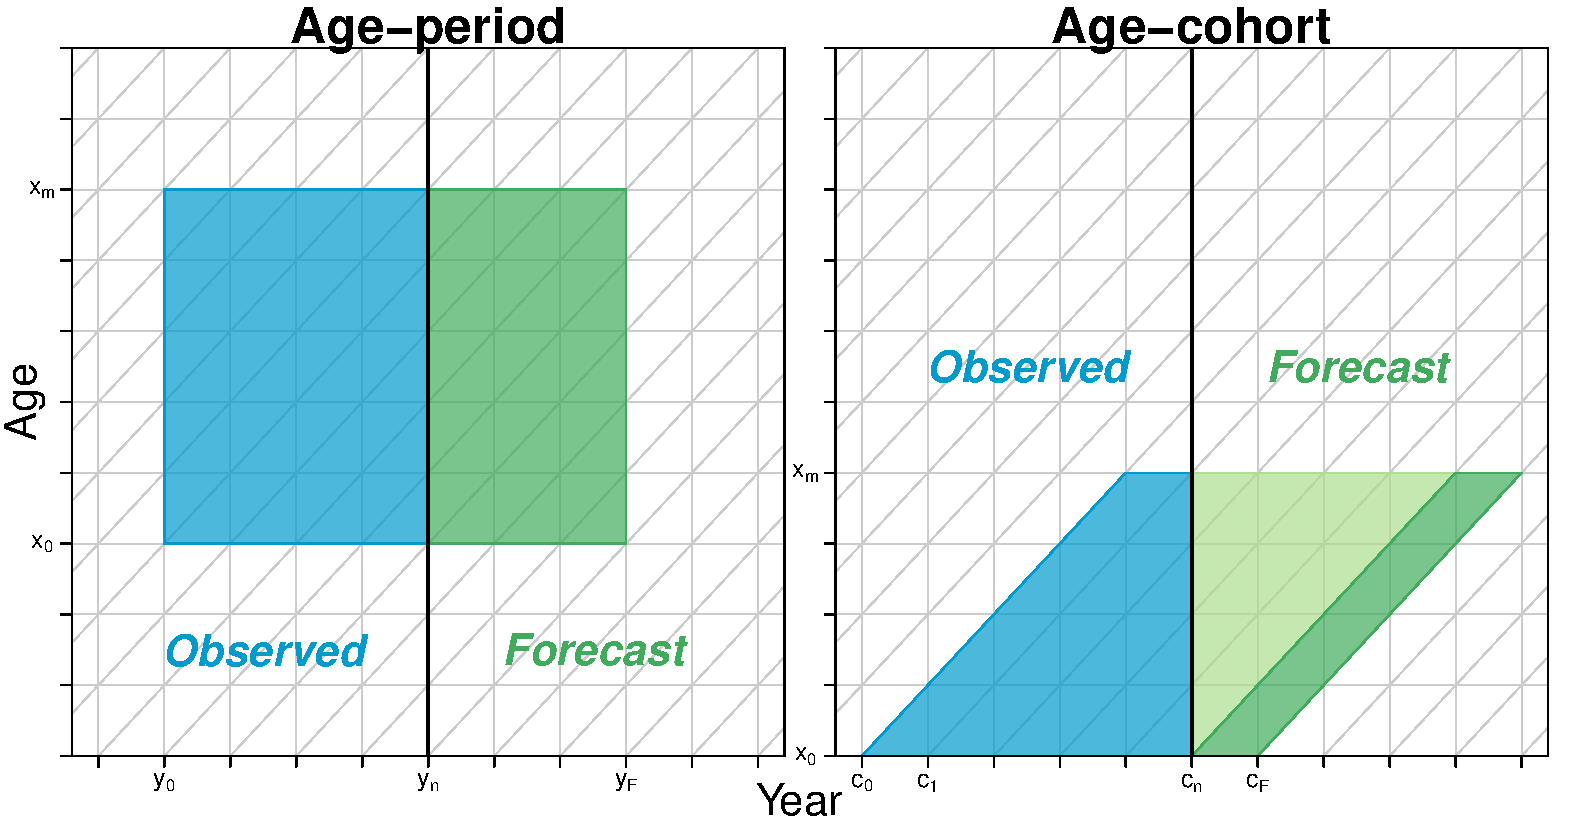
\includegraphics[scale=0.78]{./Ch3/F5.pdf} 
		\caption{Estimated and forecast STAD
			parameters $s$ (red line, top panels), $b_{L}$ and $b_{U}$ (green and blue line, respectively, bottom panels) with 80\% prediction intervals for females in Sweden, Japan, France and Denmark during the years 1980-2040.\label{Fig:ParametersEstFore}} 
	\end{center}  
\end{figure}

Figure \ref{Fig:LeFore} shows the observed and forecast remaining life expectancies at age 30 ($e_{30}$) and Gini coefficients at age 30 ($G_{30}$) with 80\% prediction intervals in the four countries for the years 1980-2040, together with the forecasts of the LM and HU models. For the STAD, the 80\% prediction intervals around the forecasts are derived from a bootstrapping procedure \citep{efron1994introduction}. 

\begin{figure}[!ht]
	\begin{center}
		
		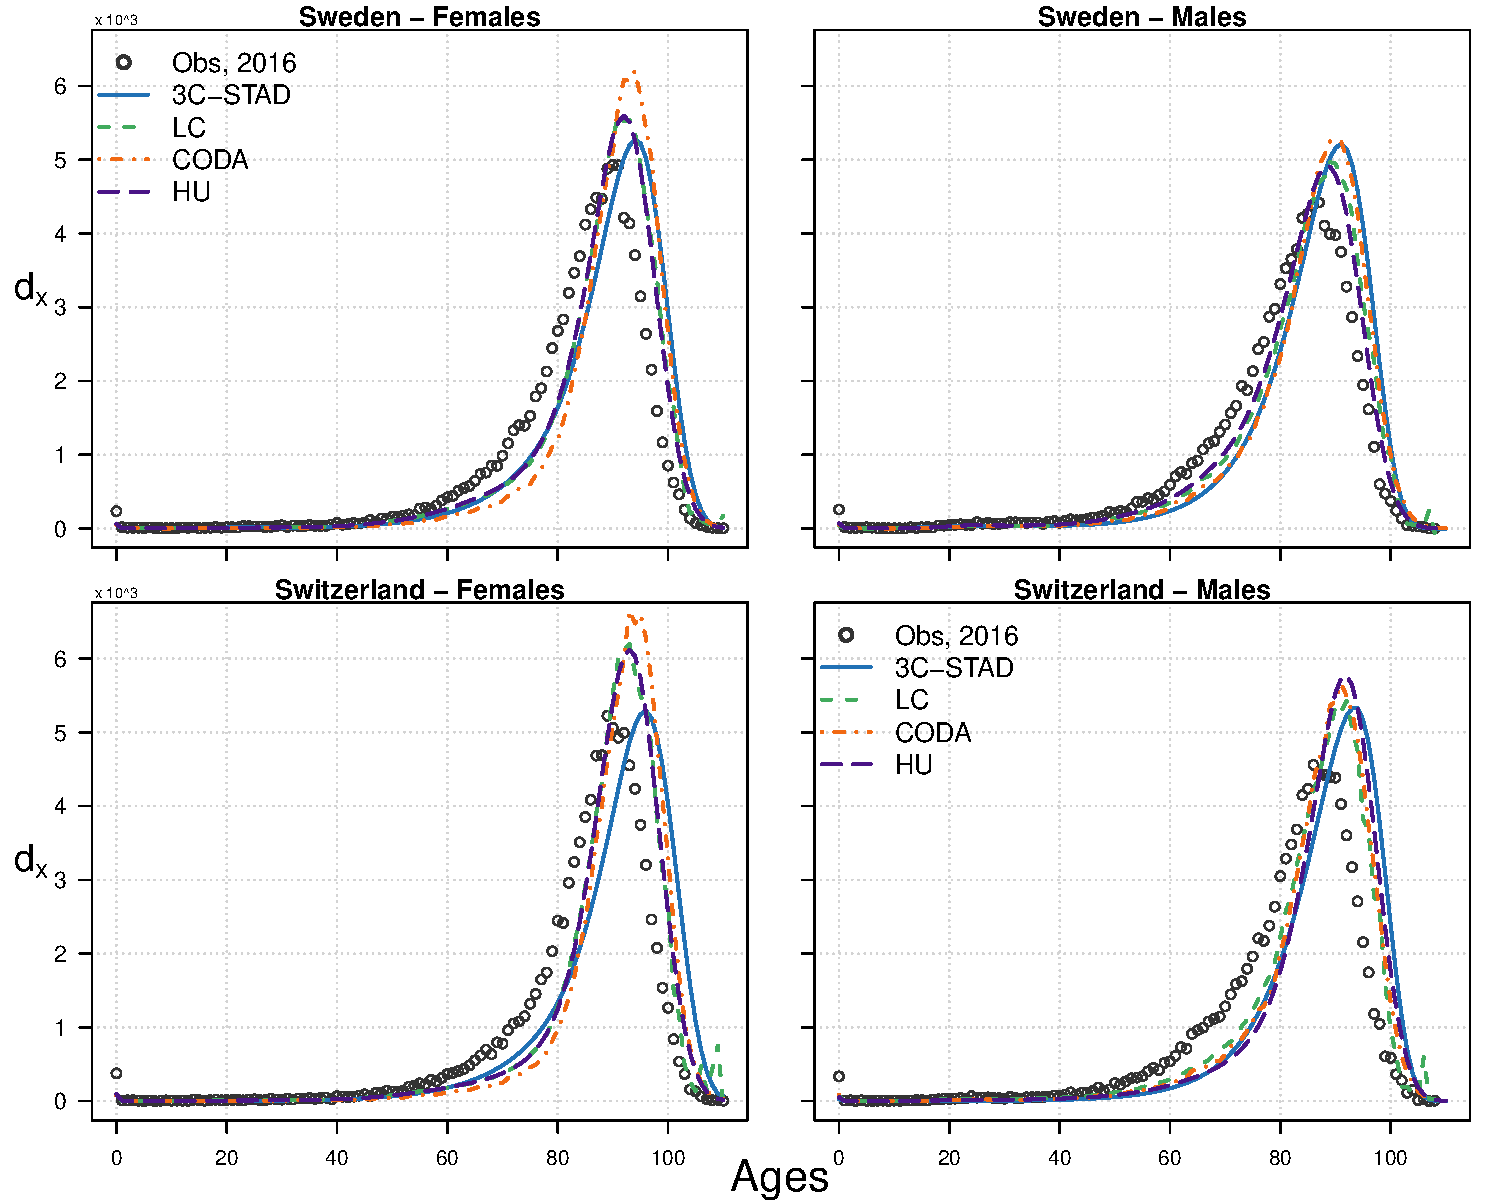
\includegraphics[scale=0.78]{./Ch3/F6.pdf}
		
		
		\caption{Observed and forecast remaining life expectancies at age 30 ($e_{30}$, top panels) and Gini coefficients at age 30 ($G_{30}$, bottom panels) for Swedish, Japanese, French and Danish females in 1980-2040 for the STAD (blue solid line and shading for the 80\% prediction intervals), LM (red dashed line) and HU (purple dashed line with dots) models.}\label{Fig:LeFore} 
		
	\end{center}
\end{figure}


The graphs of Figure \ref{Fig:LeFore} show that the STAD forecasts of $e_{30}$ reflect well the past linear increase over the years 1980-2014, and that they are more optimistic than the LM and HU forecasts. In all countries, the slope of the future increase in $e_{30}$ of the STAD is larger than those of the LM and HU model (with the exception of the HU forecast in Denmark). In Japan and France, the initial forecasts of the STAD are lower than the LC ones, but the steeper rate of increase of the STAD results in higher forecasts by 2040. With respect to $G_{30}$, the STAD forecasts generally show a slower compression of mortality than the LM and HU, most noticeably in Japan.

In Figure \ref{Fig:MxFore}, we compare the STAD, LM and HU age-specific mortality rates forecasts in 2040 for the four countries. Several differences emerge between the models from this age-pattern analysis. Mortality rates of the STAD model are smoother than the LM ones, as they are derived from a smooth standard distribution. This could be particularly advantageous for long-term projections. Discontinuities or jaggedness in the forecast age profile of mortality will be absent in the STAD forecasts, unlike in the LM model \citep{li2013extending}. Importantly, the STAD forecasts do not display the fairly unrealistic S-shape that characterizes the LM and HU forecasts for Sweden, Japan and France. In addition, the HU forecast for Denmark display an even more undulating pattern.

\begin{figure}[!ht]
	\begin{center}
		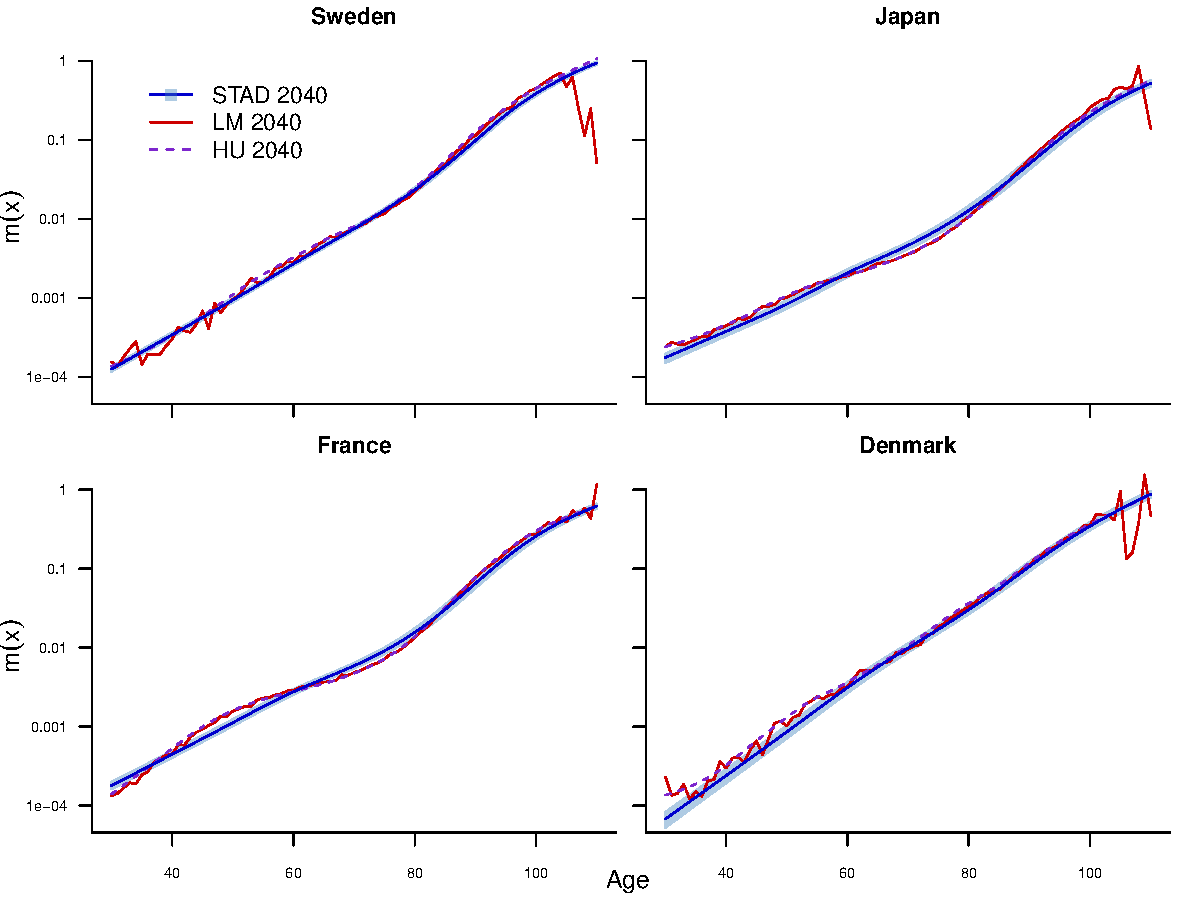
\includegraphics[scale=0.78]{./Ch3/F7.pdf} 		     
		
		\caption{Forecast mortality rates in 2040 with 80\% prediction intervals (in logarithmic scale)
			of the STAD (blue line and shading), \citeauthor{lee2001evaluating} (LM, red solid line) and \citeauthor{hyndman2007robust} (HU, purple dashed line) models for Swedish, Japanese, French
			and Danish females.\label{Fig:MxFore}} 
	\end{center}  
\end{figure}

Finally, Figure \ref{Fig:DxFore} shows the actual life-table deaths in 1980 and 2014, along with the age-at-death distributions in 2040 as computed from the STAD, LM and HU forecasts. The shifting mortality dynamic is more important and visible in the STAD model: in fact, the age-at-death distribution forecast is more shifted and less compressed than the LM and HU ones in all countries except Denmark (where the forecasts are similar).	

\begin{figure}[!ht]
	\begin{center}
		
		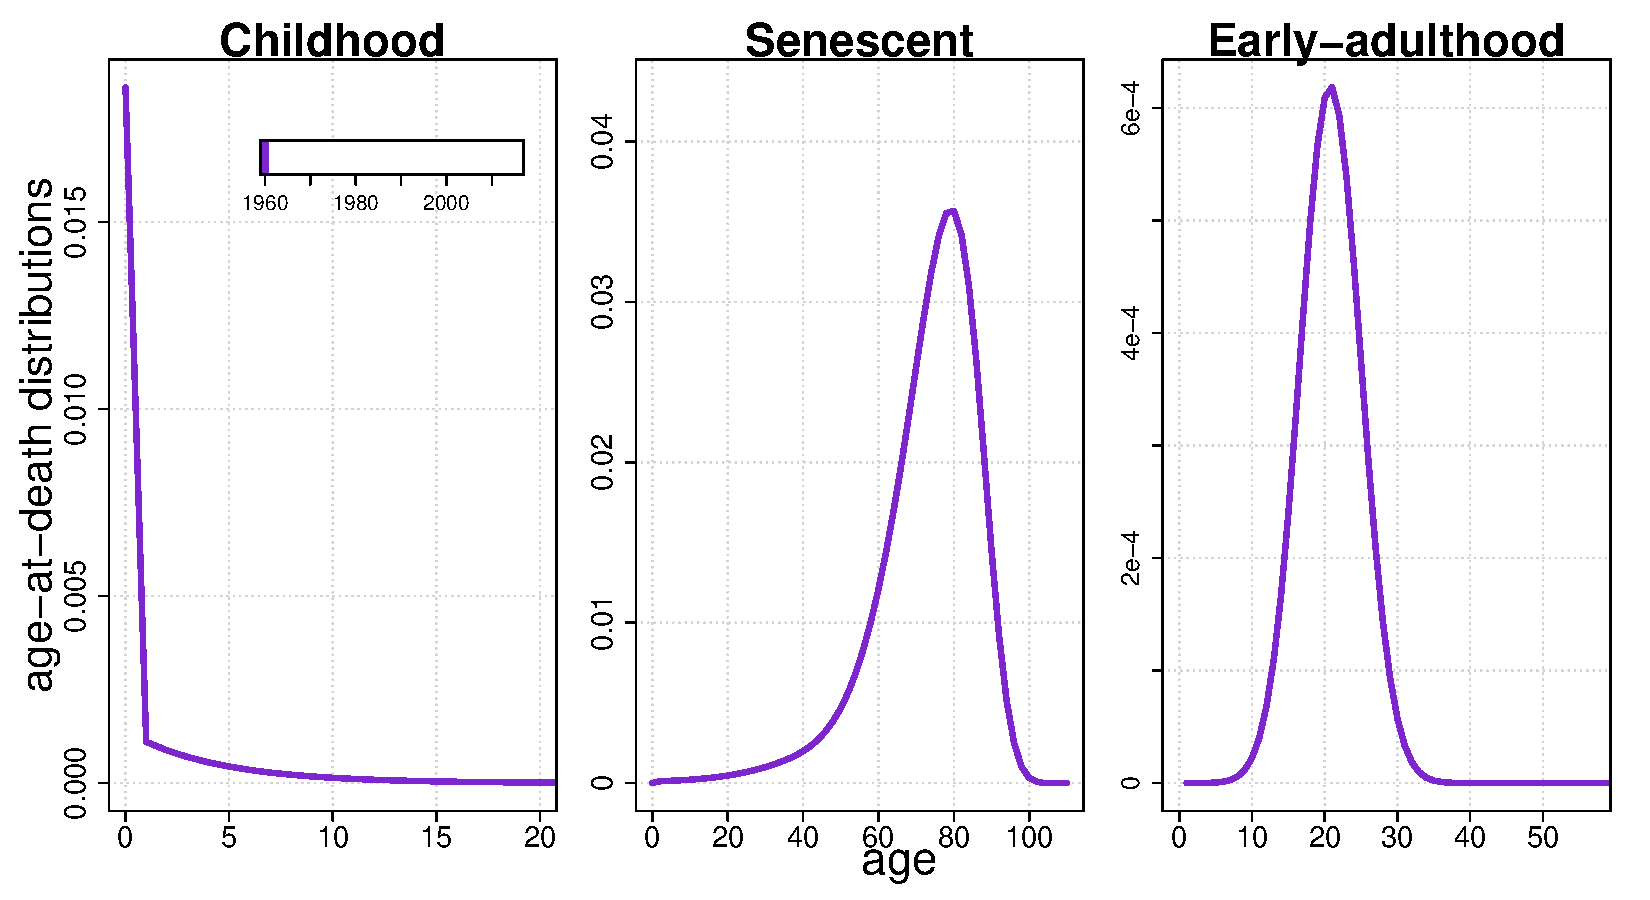
\includegraphics[scale=0.78]{./Ch3/F8.pdf}
		
		
		\caption{Observed life-table deaths in 1980 and 2014 and age-at-death distributions forecast in 2040 of the STAD (blue line and shading for the 80\% prediction intervals), \citeauthor{lee2001evaluating} (LM, red solid line) and \citeauthor{hyndman2007robust} (HU, purple dashed line) models for females in Sweden, Japan, France and Denmark.}\label{Fig:DxFore} 
		
	\end{center}
\end{figure}


\section{Discussion and conclusion}\label{Sec:Ch3sec4}

Age-at-death distributions provide a very informative description of
the mortality pattern of a population, and they are well suited
to study two important indicators of population health, namely
longevity and lifespan variation. Despite these advantages, they have
generally been neglected in modelling and forecasting human mortality,
as most techniques are based on the complementary age-specific mortality rates. 

In this paper, we propose a novel methodology for modelling and
forecasting adult mortality based on age-at-death distributions. To our
knowledge, this is one of the very first attempts in this
direction. In particular, we introduce a segmented linear
transformation model that captures mortality dynamics over time from
changes in modal ages at death and variability of the distributions
with respect to a fixed standard. This approach is both parsimonious
and revealing: using only three parameters, it enables us to portray
and forecast mortality developments, capture the compression and
shifting dynamics of mortality, and construct life-table functions.     
Given its features, we call our suggested model \emph{Segmented
	Transformation Age-at-death Distributions} (STAD). 

The results indicate that the STAD model performs very well in terms of goodness-of-fit: the estimated remaining life expectancies and Gini coefficient ($e_{30}$ and $G_{30}$) for females in four high-longevity countries (Sweden, Japan, France and Denmark) are very close to the observed historical values. Moreover, the STAD forecasts of $e_{30}$, $G_{30}$ and of the logged age-specific death rates are more accurate than the \citeauthor{lee1992modeling} (LC, \citeyear{lee1992modeling}) model and its variants in three out-of-sample validation exercises with forecast horizons of 10, 20 and 30 years. The STAD forecasts of $e_{30}$ for the four countries up to 2040 reflect well the past linear increase observed between 1980 and 2014, and they are more optimistic than the LC variants forecasts, which have often under-predicted future gains in life expectancy \citep{lee2001evaluating}. Finally, the STAD forecasts are characterized by greater shifting and smaller compression than the LC ones.

Theoretically, the STAD model can be viewed as a relational model \citep{brass1971scale}. Here, transformations of a standard age-at-death
distribution $f(x)$ describe mortality developments \emph{over time}
rather than across countries. From this perspective, an analogy can be
made between the STAD and the LC model. The series of $\alpha_x$ in the LC can be viewed as a
standard mortality age-profile, whose development over time is
captured by the index $\kappa_t$ modulated by a fixed rate of mortality improvement at age $x$, $\beta_x$. As such, the LC model can also be interpreted as a relational model. 

Our methodology is also inspired by the model proposed by
\cite{camarda2008warped} to analyse mortality developments from
age-at-death distributions by transforming the age axis with a smooth
non-linear warping function. Furthermore, \cite{cadena2016semi}
recently introduced an accelerated hazard relational model based on a
smooth transformation of the age scale free of monotonic
constraints, and they used it to estimate and project mortality in
Belgium. The STAD model has elements that are common to both
approaches, but it is also significantly different. The first model
has been developed for mortality analyses, and the smooth function is
not well suited for forecasting. The second model is based on the
hazard function, and is subject to the same characteristics as models
based on mortality rates discussed in the Introduction. 

As in most relational models, the choice of the standard is important:
all the features contained in $f(x)$ are in fact carried in the
transformation function $t(\cdot)$. In order to maximize the
representativeness of the standard with respect to the observed
densities, we choose $f(x)$ as the mean of the aligned distributions, employing a landmark registration approach inspired from
Functional Data Analysis \citep{ramsay2005FDA}. With this technique,
the ages occurring before and after the modal age are no longer
conflated: differences in the mode (that are already accounted
for by the parameter $s$) are removed, and the focus is only on differences in variability of the distributions. The use of functional data
techniques in modelling and forecasting mortality already has other
precedents in the literature
\citep{hyndman2007robust,hyndman2008stochastic,hyndman2013coherent}. 

The shifting and compression dynamics of mortality changes have been
investigated extensively in recent decades \citep[for
example,][]{fries1980aging,kannisto2000measuring,bongaarts2002long,bongaarts2005long,canudas2008modal,thatcher2010compression,bergeron2015decomposing,de2016new}. In most developed countries, a compression of mortality was observed
during the first half of the twentieth century. In the second half of
the century, the compression dynamic was mainly replaced by the
shifting of the mortality schedule, with lifespan variability
remaining practically constant. In addition to capturing longevity and
lifespan variability changes, the three parameters of the STAD model
provide information on these two dynamics. The parameter $s$ regulates
the shifting dynamic, as it measures the change in the modal age at
death over time. The parameters $b_L$ and $b_U$ regulate the
compression dynamic, as they expand or reduce the variability of
deaths before and after the mode with respect to the standard
distribution. These two parameters disentangle the 
contribution to the compression dynamic of two groups of people: those
younger and those older than the modal age.  This decomposition brings new evidence on the compression dynamic, adding a novel perspective to this stream
of research \citep{fries1980aging,myers1984compression,wilmoth1997search,wilmoth1999rectangularization,lynch2001reconsidering}.

The STAD model can thus be used to study the developments of the shifting and compression dynamics over a specified time interval, and this analysis can in turn usefully inform mortality projections. Appropriately accounting for these different dynamics in projections is a desirable property for forecasting mortality. For example, our analyses on females in four high-longevity countries between 1980 and 2014 suggest that the shifting dynamic has played a very important role in mortality patterns \citep[as it has been observed elsewhere, for example][]{canudas2008modal,bergeron2015decomposing,de2016new}. Compared to the LC model, the age-specific pattern of the STAD forecasts is characterized by a greater shift in all countries, as reflected in the age-at-death distribution forecast. Similar results have been shown for the Netherlands, using a new parametric model that considers both shifting and compression \citep{janssen2016projecting}.


From a survival analysis perspective, the STAD model can be linked to
the class of \emph{accelerated failure time} (AFT) models. In survival
analysis, AFT models have been introduced as an alternative to
proportional hazard regression models to describe the effects of
covariates in accelerating or decelerating the ageing process
\citep{wei1992accelerated,kalbfleisch2002statistical}. The STAD model
can be interpreted as a particular type of AFT model, in which the
ageing process is not uniformly modified with respect to the reference
(the standard distribution), but it is rather modified in different
ways before ($b_L$) and after ($b_U$) the modal age at death. For
example, the ageing process could be accelerated before and
decelerated after the mode with respect to the standard, or
vice-versa, or accelerated/decelerated at different rates in the two
age segments. 

From this perspective, one limitation of the STAD model lies in the difficulty of interpreting its result from the individual standpoint. It is quite unrealistic to hypothesize that all individuals of a population age at two different rates, one before and one after the overall modal age at death. However, our aim here is to introduce a novel approach for modelling and forecasting mortality at the population level. The assumption of different rates of ageing can
be more easily justified from this aggregate perspective, as the two parameters capture the \emph{average} ageing rate in the two well-characterized age segments of the population. Nevertheless, while no experiments have been performed with medical and epidemiological datasets, the STAD might be unsuitable as a regression model for the analysis of
survival data, and a completely smooth transformation function, as in \cite{camarda2008warped}, might be preferable. Furthermore, an additional limitation of the STAD model, as of all other models employed here, is that cohort effects are neither considered nor modelled. Analysis of cohort data is currently foreseen as future work.

Our interest in this article is limited to the senescent (older adult) mortality pattern, and our analyses start from age 30. Applying the STAD model to the entire age range reduces fitting accuracy. The reason for this loss of accuracy lies in the
shape of the human mortality pattern. Since
\cite{thiele1871mathematical}, demographers use to decompose the mortality
age-profile into three different groups operating
principally, or almost exclusively, upon juvenile, younger adult and
older adult ages. Applying the model
from age 30 produces satisfactory results for the female populations analysed in this article because the first two components are negligible with respect to the senescent component. For males, the STAD model produces satisfactory results too (analyses not shown here), although the goodness-of-fit is slightly reduced compared to females. This is because the assumption that the younger adult mortality component (the accident hump) is negligible at age 30 is probably too strong for males. More accurate results for males could be obtained by extending this work to model and forecast the entire mortality pattern by: (i) disentangling
and estimating the three independent age-specific mortality components
and (ii) applying the STAD model, or a modified version of it, to each component. The Sum of Smooth
Exponentials model \citep{camarda2016sums} can be thought as a
starting solution for the former issue. 

We conclude with one last remark on our STAD model. We have chosen the
modal age at death as the break-point of the segmented linear
transformation because several demographic studies aforementioned
investigated the variability of deaths after the modal age at
death. In this respect, we add to this literature by studying the
variability before and after the mode \emph{simultaneously}. However,
any other age of the distribution can be chosen as break-point,
for example one of the other two central tendency measures (the mean
and the median age). In practice, this might be more appropriate for
studying mortality in countries with data deficiencies or for the analysis of
causes of death, and this approach will be explored in future work. 

% ---- Appendix ----
% --------------------------------------------
\section{Appendix}\label{Sec:Ch3Appendix}

\subsection{Deviance, Effective Dimension and BIC}\label{Subsec:Ch3appA}

The Deviance is often used as a measure of discrepancy between observed and fitted data. Within a Poisson framework, it is defined as:   
%
\begin{equation}
\mathrm{Dev}= 2 \sum_{y} \sum_{x} \left[D_{x,y} \, \ln \left( \frac{D_{x,y}}{\hat{D}_{x,y}}  \right) - (D_{x,y} - \hat{D}_{x,y} )\right] 
\end{equation}
%
where $D_{x,y}$ and $\hat{D}_{x,y}$ denote the observed and fitted
number of deaths at age $x$ and year $y$, respectively. Higher values
of the Deviance correspond to worse models in terms of goodness-of-fit. 

The Bayesian Information Criterion \citep[BIC,][]{schwarz1978estimating} is frequently employed to assess model differences in terms of trade-off between model parsimony and accuracy. In a two-dimensional age and time setting, the BIC can be computed as: 
%
\begin{equation}
\mathrm{BIC}=\mathrm{Dev} \, +  \, \ln(m n)  \, \mathrm{ED}
\end{equation}
%
where $m$ and $n$ are the dimensions (length) of age and time,
respectively. ED denotes the Effective Dimension, or total number
of parameters, of a model. Lower BIC values are associated with better
models, and the trade-off between accuracy and parsimony is accounted
for by the two components of the BIC. 


\subsection{Sec.~\ref{Subsec:Ch3subsec3.1}: additional results}\label{Subsec:Ch3appB}

Here, we present the Deviance and Effective Dimension (ED) of the STAD model and LC variants corresponding to the analysis of Section \ref{Subsec:Ch3subsec3.1}. Table \ref{Table:DEV} shows the Deviance values of the STAD and LC variants in the four countries, and the ED of each model is reported in Table \ref{Table:ED}. 

In terms of the Deviance, the \citeauthor{hyndman2007robust} method (HU) is the best fitting model, as its Deviance is always smaller than those of other models. Among others, one explanation for the improved fit of the model with respect to the STAD and other LC variants is that the HU model employs a very high number of parameters: almost four times more than the LC (765 versus 195) and five times more than the STAD (765 versus 138). This high parameterisation is penalized by the BIC measure, so that the HU model is the optimal choice in only one instance (Japan, see Table \ref{Table:BIC}). In terms of parsimony, the STAD model is the best performer, as it employs less parameters than the other models.

% % DEVIANCE

\begin{table}[!ht]
	\centering
	
	\begin{tabular}{lR{1.4cm}R{1.4cm}R{1.2cm}R{1.2cm}R{1.4cm}R{1.4cm}R{1.4cm}R{1.4cm}}
		\toprule
		& \multicolumn{8}{c}{Model} \\ \cmidrule(rr){2-9} 
		Country & STAD & LC & LM & BMS & BDV & HU & HUrob & HUw           \\ 
		\rowcolor{my-grey}
		\midrule
		\belowrulesepcolor{my-grey}
		Sweden                   & 3179          & 3149           &     3153      & 3123       & 3060  & \textbf{2789}   & 2958     &   2936    \\ 
		
		Japan                    & 9962          & 9925                &     10268      & 9837        & 9240   & \textbf{3975  }  & 4612     &   4900         \\
		\rowcolor{my-grey}
		France                   & 8046          & 6272                 &     6400        & 6223        & 6113 & \textbf{3320}    & 4050      &   3776 \\
		Denmark                  & 4235          & 4063   &     4054      & 4036     & 3934      & \textbf{2938} &  3316     &   3808            \\ 
		\bottomrule
	\end{tabular}
	\caption{Deviance values of the STAD and LC model and variants for females aged 30-110+ in four countries during 1980-2014. Lower values of the Deviance (in bold) correspond to a better fit to the data.}\label{Table:DEV}
\end{table}


% % EFFECTIVE DIMENSION
\begin{table}[!ht]
	\centering
	
	\begin{tabular}{lR{1.4cm}R{1.4cm}R{1.2cm}R{1.2cm}R{1.4cm}R{1.4cm}R{1.4cm}R{1.4cm}}
		\toprule
		& \multicolumn{8}{c}{Model} \\ \cmidrule(rr){2-9} 
		Country & STAD & LC & LM & BMS & BDV & HU & HUrob & HUw           \\ 
		\rowcolor{my-grey}
		\midrule
		\belowrulesepcolor{my-grey}
		Sweden                   & \textbf{138}         & 195           &     195      & 195        & 195  & 765   & 765   &   765    \\ 
		
		Japan                    & \textbf{138}          & 195          &     195     & 195       & 195 & 765   & 765    &   765        \\
		\rowcolor{my-grey}
		France                   & \textbf{138}          & 195                &     195     & 195       & 195 & 765  & 765    &   765 \\
		Denmark                  & \textbf{138}         & 195           &     195            & 195        & 195    &  765  & 765    &    765               \\ 
		\bottomrule
	\end{tabular}
	\caption{Effective Dimension (ED, total number of parameters) of the STAD and LC model and variants for females aged 30-110+ in four countries during 1980-2014. Lower ED (in bold) corresponds to a more parsimonious model.}\label{Table:ED}
\end{table}

\cleardoublepage

\end{document}